% 段落IDはsections_en.texに対応する。
\begin{abstract}
% P:abstract
測定した特化が似ている二つの学習器は、同じ新しい学習条件に異なる応答を示すだろうか。本研究では、形成履歴と最適化器状態を制御できる小規模な共有表現ネットワークによって、この問いを調べる。異なる観測・損失重み履歴から、平均再構成測定値が同等な状態を作る。他方の対象を優位にする共通介入では、10更新以内に、より精密に読み出せる対象が入れ替わるチェックポイントの割合は、取得形成で67.5\%、更新形成で0\%となる。Adamを初期化すると、再配分量の経路間差は事前に定めた同等幅内まで縮小する。独立した成分交換実験では、二次モーメントの交換によって、どちらの履歴が変化しやすいかが逆転する。さらに、平均的な適応倍率と座標別の配置を分けて介入すると、平均倍率を揃えることで差は減り、その共通倍率の下で配置を交換すると符号が変わる。新規Adamと校正SGDでは小さな差が遅れて現れ、共通の学習を続けると、500更新までに配分終点は近づく。したがって、測定した特化の背後に、二次モーメント構造を因果的な修飾要因とする、逆転可能な短時間適応差が隠れていることがある。終点を揃えた比較は、二つの容量の三Gaussian対象へ拡張できた。三室の実測センサデータでも成分効果は残ったが、終点一致は満たさず、隠れた感受性についての証拠の範囲が明確になった。
\end{abstract}

\section{序論}
% P:intro1
共有表現とは、複数の予測課題が利用する内部符号である。容量が限られると、ある課題に役立つ情報が、別の課題の情報より復元しやすい状態で残ることがある。この読み出し精度の不均等を\emph{表現特化}と呼ぶ。このような偏りはすでに知られており、特徴の複雑さ、学習順序、情報源間の競合が、ネットワークの表現する内容を変えうる\citep{lampinen2024biased,pezeshki2021gradient,huang2022modality}。本研究では、測定した特化から、学習条件が変わった後の学習器の応答について何が分かるかを問う。

% P:intro2
この問いは、性能を評価した後にもモデルが学習を続ける場面で重要になる。現在は同程度の予測を支える二つのモデルでも、共有特徴を再配分するために必要な学習量は異なるかもしれない。学習履歴は、モデルのパラメータと最適化器状態の両方を通じて、新しい情報から学ぶ能力、すなわち可塑性に影響する\citep{achille2019critical,lyle2023plasticity,dohare2024plasticity}。実験上の課題は、現在測定した能力の違いと、その後の応答の違いを区別し、さらに応答を変える持続状態成分を同定することである。

% P:intro3
二つの経路で特化を形成し、この比較を構成する。一方は再構成誤差を等しく重みづけしながら一方の対象を精密に観測し、他方は精密な観測を均衡させながら、その対象の誤差を重く扱う。パイロット校正により、選択した平均終点測定値を固定した許容幅内で同等にする。その後、反対の対象を優位にする同じ介入を加える。これらの測定値が、この介入下の適応を十分に特徴づけるなら、両経路は似た応答を示すはずである。引き継いだ最適化器状態が、測定からは見えない応答差に寄与するなら、介入開始時の各モデル重みを固定したまま、その状態を初期化・交換することで対比が変わるはずである。

% P:intro4
結果は、大きな初期応答差について後者の説明を支持する。Adamの二次モーメントは、勾配の二乗を逐次平均した量であり、パラメータごとに更新倍率を調整する。これを交換すると、どちらの形成経路が大きく変化するかが逆転する。平均逆倍率を揃えても応答差は残り、共通平均倍率の下で座標別配置を交換すると符号が変わる。これらの介入は、適応倍率の配置が受容側ネットワークの再配分をどう変えるかを同定する。さらに長い軌道は、観測時間が重要な理由を示す。引き継いだAdam状態を除去しても小さな経路差が後から現れ、共通の学習を長く続けると、測定した配分終点は近づく。

% P:intro5
本研究の実証的貢献は、つながりを持つ三点からなる。選択した再構成測定値を揃えた後の適応比較、短時間応答差を変える成分・倍率・配置への介入、そして引継ぎ状態による大きな一過性の差と小さな遅発差を区別する時間比較である。これらの終点測定に隠れた応答差を、\emph{潜在的感受性}と呼ぶ。小さな人工学習器を用いることで、対応づけた履歴、保存モデル状態、最適化器成分を必要な粒度で制御できる。終点を揃えた比較は二・三対象のGaussian系を含む。実測センサデータでは、対象間の関係と時間変動がある場合にどの部分が残るかを検証する。相補的な形成・維持実験は、特化の広い過程の中にこれらを位置づける。

\section{学習履歴と最適化器の記憶に関する先行研究}
\label{sec:related}
% P:related1
測定した性能が似ていても、予測器間に重要な違いが残ることは、過少特定の問題として研究されている\citep{damour2022underspecification}。表現類似度の測定は、終点の別の側面を調べる\citep{kornblith2019similarity}。本研究の比較対象は追加学習への応答であり、共通介入の前に選択した再構成測定値を揃える。この比較は、初期経験と学習過程が後の学習を変える可塑性研究につながる\citep{achille2019critical,jastrzebski2020breakeven,dohare2024plasticity}。

% P:related2
最適化器が媒介する履歴効果には、直接の先行研究がある。\citet{lyle2023plasticity}は可塑性を損失形状と関連づけ、課題変化後にAdamのモーメント推定が異なる速度で追随することが、学習を不安定にしうると示す。\citet{asadi2023resetting}は、強化学習の目的が変わった後の最適化器初期化を評価する。\citet{ellis2024local}は、勾配規模が変わった後の更新幅の過渡変化を解析し、相対的なAdam時刻を導入する。これらの結果から、引き継いだ適応倍率が、本研究で確かめる具体的な説明候補となる。問うのは、\emph{表現の再配分}における経路差を平均倍率で十分に説明できるか、それとも座標別配置も差を変えるかである。

% P:related3
隠れた学習効果を調べるために、状態を直接移植する研究もある。最近のプレプリントで\citet{xu2026optimizer}は、潜在的な特性転移を運ぶ一次モーメントを同定する。直後の出力に現れない介入が、その後の学習中に差を生む。\citet{sevetlidis2026trainingmemory}は履歴の保持先を整理し、状態に基づく因果的測定を提案する。本研究が加えるのは、共有表現の適応についての具体的な実証的分解である。再構成測定値の調整、二次モーメントの倍率・配置介入、引継ぎAdam・新規Adam・SGDでの共通継続を組み合わせる。最も近い比較を表\ref{tab:prior}にまとめる。

\begin{table}[t]
\centering\small
\caption{最も近い先行比較と、本研究で検証する問い。介入と測定結果を対応づけ、比較同士の関係を示す。}
\label{tab:prior}
\begin{tabularx}{\textwidth}{>{\raggedright\arraybackslash}p{.21\textwidth}>{\raggedright\arraybackslash}X>{\raggedright\arraybackslash}X}
\toprule
先行研究 & 確立された比較 & 本研究の比較\\
\midrule
\citet{lyle2023plasticity} & 変化する課題における可塑性、損失形状、最適化器の不安定性 & 選択した再構成測定値を揃えた後の再配分応答\\
\citet{asadi2023resetting,ellis2024local} & 状態・時刻の初期化と、目的・勾配規模変化による更新幅への影響 & 成分交換と、平均逆倍率を揃えた座標配置\\
\citet{xu2026optimizer} & 直後の出力不変性を含む、一次モーメント移植と後の転移 & 二次モーメント構造と特化応答の時間経過\\
\bottomrule
\end{tabularx}
\end{table}

% P:related4
これらの研究は学習状態の重要性を示すが、測定する結果は異なる。10更新パルスによる特化の変化は、最適化性能の改善とも、蓄積した特性転移の測定とも異なる。一次モーメント交換による応答対比の変化の区間は、この観測時間では事前の同等幅内にあった。長い軌道では、共通の反対課題において再配分の効果がどこまで続くかを検証する。別の下流課題への学習属性の転移は、今後の比較課題である。

\section{特化と適応を比較する制御実験}
\label{sec:approach}
\subsection{一つの共有ボトルネックを通る二つの形成経路}
% P:design1
中心となる学習器は、雑音を含む観測から二つの三次元信号$A$と$B$を再構成する。標準ガウス分布から$A$と独立な$\epsilon$を生成し、$\rho=0.35$として$B=\rho A+\sqrt{1-\rho^2}\epsilon$とする。seedごとの直交変換で観測を混合する。各層の後にtanhを置いた$6\to32\to2$エンコーダが、観測を二つの数値からなる符号へ写し、二つの線形再構成ヘッドがそれを共有する。学習対象は雑音のない信号である。このボトルネックにより、読み出せる情報の配分を観測できる。

% P:design2
情報品質と誤差の重みづけを別々に操作する。\emph{取得精度}は混合前の対象別入力雑音を変え、高精度・低精度の標準偏差は0.05と1.20である。各雑音チャネルを$\sqrt{1+\sigma^2}$で割り、分散を正規化する。\emph{更新配分}は再構成損失の重みを変える。
\begin{equation}
L_t=w_{A,t}\ell_{A,t}+w_{B,t}\ell_{B,t},\qquad w_{A,t}+w_{B,t}=1.
\label{eq:loss}
\end{equation}
重みを等しくすると、誤差の明示的な重要度は等しくなるが、勾配は異なりうる。したがって、観測品質は損失重みとは異なる介入を通じて学習へ入る。関連研究は能動的取得と課題重みづけを扱う\citep{shim2018joint,chen2022active,chen2018gradnorm,yu2020gradient}。本設計は、一つの共有表現でこれらの制御を交差させる。

% P:design3
均衡した100初期化更新の後、取得と重みづけの九条件比較を500更新行い、各制御がどちらの対象を優位にするかを調べる。均衡取得は、各対象に高精度更新を正確に250回ずつ割り当てる。終点を揃える比較では、取得経路は等損失重みで優位対象を精密に観測し、更新経路は取得を均衡させ、優位対象に重み0.80を与える。経路強度はパイロットseedで校正し、確認実験では固定する。形成・移行の全対照は\ref{app:formation}に示す。

\subsection{共通測定と対応づけた推論}
% P:design4
読み出せる情報を測るため、エンコーダを固定し、未使用プローブデータで新しい線形読み出し器を当てはめ、別の未使用データで評価する。両対象に共通の高精度入力を与える。分散で正規化した平均二乗誤差を$D_A,D_B$とする。配分指数
\begin{equation}
s=\frac{D_B-D_A}{D_A+D_B}
\label{eq:s}
\end{equation}
は、$A$をより精密に読み出せるとき正になる。元の優位対象へ符号を揃えると、その低下が他方への再配分を測り、ゼロ交差は読み出しやすい対象の入れ替わりを示す。両誤差、その和、共通低精度プローブ下の配分も保持する。したがって、相対的な優位を絶対的な再構成品質とともに評価する。

% P:design5
各seedで共通の起点と対応づけた入力・雑音系列を用意する。条件は同じ初期モデルから分岐し、操作しない限り最適化器状態も共通とする。パイロットと確認seedは重複せず、各主要比較に40確認seedを用いる。推論では鏡像の対象ラベルをseed内で平均し、95\% seedブートストラップ区間を報告する。終点の同等性は、対応差の平均の区間が各事前許容幅内に入ることを要求するもので、全ペアの測定値が同一という主張ではない。全確認seedを保持する。形成後のモデルパラメータと表現の幾何形状は異なりうる。

% P:design7
各計画では、確認実行前に、配分指数または正規化誤差の単位で許容する平均差の上限を固定する。\ref{app:optimizer}に、測定値を揃える許容幅と応答の同等幅、および別に設けたパイロット段階を示す。

% P:design6
中心証拠は、終点調整実験（IV-D）、独立した成分交換と経路内対照（IV-E）、さらに新規40 seedによる倍率・配置と時間経過の事前固定追試からなる。補助実験は、形成（IV-B）、移行（IV-A/C）、維持（II/III）、三対象形成（V-A）を扱う。三対象適応（V-B）と実測センサ比較（V-C）は、新しいseedで成分効果の適用範囲を検証する。\ref{app:optimizer}に正確な介入と全推定値を示し、\ref{app:status}で事前指定検証、探索的解析、不成立の候補を区別する。

\section{揃えた特化に短時間の応答差が隠れている}
\label{sec:latent}
% P:response0
どちらの制御も特化を選べる。等損失重みの下で$A$または$B$を精密に取得すると、平均配分指数は0.3385と$-0.3338$となり（図\ref{fig:headline}a）、反対側への十分に強い更新重みは、この取得による優位を上回りうる。

% P:response1
二つの形成経路は、測定上似た特化へ到達する。符号を揃えた$s$、対象・非対象誤差、総誤差、低精度の符号を揃えた$s$という五つの終点基準をすべて通過する。符号を揃えた$s$の平均差は$-0.0064$（$[-0.0098,-0.0032]$）で、$\pm0.02$内にある。均衡観測・等重みの中立継続200更新にわたる平均積分応答も、引継ぎAdamと新規Adamのどちらでも同等である。したがって、選択した静的測定値と一つの中立継続要約を揃えたうえで、反対条件への応答を検証できる。

% P:response2
各形成済み学習器を、10更新からなる三つの反対介入へ複製する。取得だけのパルスは、等損失重みで、それまで読みにくかった対象を精密に観測する。更新だけのパルスは取得を均衡させ、その対象へ重み0.80を与える。複合パルスは、その対象を精密に観測して重み0.85を与える。各パルスを引継ぎAdamと新規初期化Adamで検証し、分岐時の受容側モデル重みは固定する。応答は符号を揃えた$s$の低下量、経路対比は取得形成の低下量から更新形成の低下量を引いた値である。

\begin{figure}[t]
\centering
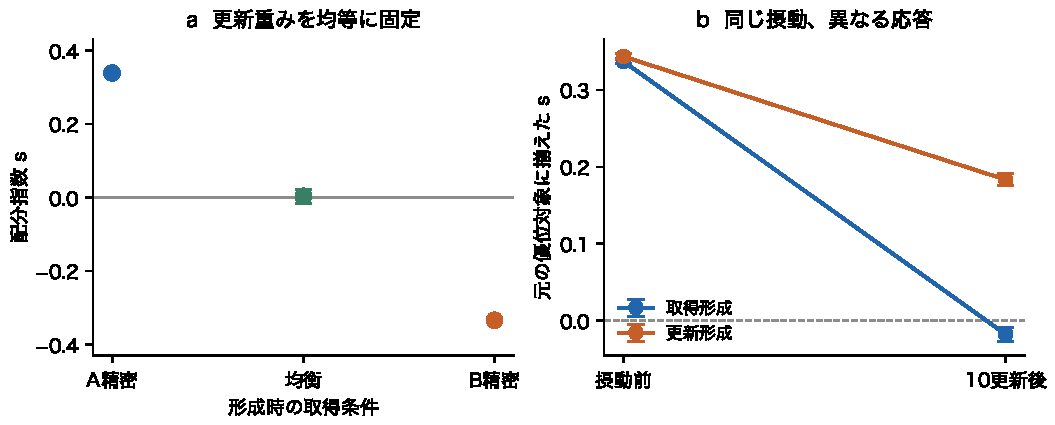
\includegraphics[width=.88\textwidth]{../figures/headline_ja.pdf}
\caption{共通の測定配分の背後に、異なる適応が隠れうる。(a) 等損失重みで取得が特化を選ぶ。(b) 終点を揃えた形成経路に、同じ複合反対パルスを与える。両者とも反対対象へ動くが、取得形成経路の変化が大きい。点と区間は40 seedを要約し、(b)の鏡像ラベルはseed内で平均する。線は途中の軌道ではなく、終点を結ぶ。}
\label{fig:headline}
\end{figure}

% P:response3
Adamを引き継ぐと、すべてのパルスで取得形成経路の変化が大きい（表\ref{tab:pulses}）。複合パルスでは、そのcheckpointの67.5\%が10更新以内にゼロを越えるのに対し、更新形成では0\%である（図\ref{fig:headline}b）。連続的な経路差は0.1951である。Adamを初期化すると0.0103へ減り、事前の$\pm0.02$幅内に入る。他のパルスでも同様に減少する。したがって、引き継いだ最適化器状態は、選択した終点測定と中立継続には現れなかった応答差を大きく変える。

\begin{table}[t]
\centering\small
\caption{反対条件10更新後の特化低下量の経路差。角括弧は95\% seedブートストラップ区間を示す。引継ぎ条件の全区間は$+0.05$より上、初期化条件の全区間は$\pm0.02$内にあり、それぞれの事前基準を満たす。}
\label{tab:pulses}
\begin{tabular}{lcc}
\toprule
パルス & Adam引継ぎ & Adam初期化\\
\midrule
取得のみ & $0.1668\ [0.1601,0.1736]$ & $0.0011\ [-0.0010,0.0035]$\\
更新のみ & $0.1510\ [0.1456,0.1562]$ & $0.0120\ [0.0093,0.0149]$\\
複合 & $0.1951\ [0.1880,0.2021]$ & $0.0103\ [0.0079,0.0129]$\\
\bottomrule
\end{tabular}
\end{table}

% P:response4
この結果は、二対象ネットワークと10更新パルスに適用される。別途測定した線形な表現類似度（CKA）の平均は0.927であり、モデルパラメータは同一ではない。Adamを初期化しても、これらのモデル差は残る。したがって小さな初期化対比が示すのは、この時間での限定された応答同等性であり、表現の同一性ではない。ゼロ交差率も短いパルスを記述する。第\ref{sec:time}節で、より長い共通学習を調べる。

% P:endpointprediction
既存の三つの40 seed集合を用いた探索的検査では、seed内に残る終点差が応答対比を予測するかを調べた。標的誤差、他方の誤差、低精度配分指数を使う線形モデルは、学習用標本の平均を予測する基準をほとんど改善しなかった。この結果は、測定した終点特徴の予測力が限られることを支持する。付録~\ref{app:extension}に未使用標本での誤差と条件付き推定値を示す。

\section{二次モーメント構造が再配分を因果的に変える}
\label{sec:mechanism}
\subsection{成分交換によって経路対比が逆転する}
% P:mechanism1
Adamは、符号付き勾配の平均$m$と、勾配の二乗の平均$v$を保持する\citep{kingma2015adam}。後者はパラメータごとの適応倍率を定める。これらを直接検証するため、受容側の重みと最適化器の更新回数を固定し、経路終点間で$m$または$v$を交換する。両経路は同じ起点から分岐しているため、パラメータ座標を対応づけられる。

% P:mechanism2
独立した40 seed比較では、$m$交換による平均応答対比の変化は小さく、事前許容幅内にある。$v$を交換すると、経路対比は$+0.1968$から$-0.1265$へ変わる（図\ref{fig:moments}a）。両推定値の区間は、互いに反対側でゼロを除く（\ref{app:optimizer}）。したがって、受容側の二次モーメント状態は、どちらの経路が変化しやすいかを変える。この介入が同定するのは、受容側の重みと後続の勾配とともに働く因果的な修飾要因であり、測定対象は複合パルス10更新の応答である。

\subsection{平均倍率は短時間応答差の一部を説明する}
% P:mechanism3
交換結果から、より具体的な問いが生じる。一方の経路は、単に平均的な適応倍率が大きいだけなのだろうか。新規40 seedの事前固定追試では、引継ぎ状態の対比は0.1907となり、先の推定値0.1951と0.1968が再現する。Adamのバイアス補正済み二次モーメント逆倍率を、パラメータ間で平均した量を$\bar a_v$と定義する。これは$v$が与える倍率であり、実際の更新は一次モーメントと現在勾配も利用する。

% P:mechanism4
各経路の座標配置を保ちながら$\bar a_v$を揃えると、応答差は0.1907から0.0875へ減る。配置を一つのスカラー値に置き換えると0.1251、スカラー化と共通倍率を組み合わせると0.0395となる（図\ref{fig:timecourse}a）。$\bar a_v$を共通に保って他経路の配置へ交換すると、差は$-0.0110$へ変わる。したがって、平均倍率は応答対比の一部を説明し、その共通平均の下でも座標配置が受容側の応答を変える。この比較で揃えるのは平均逆倍率であり、パルス全体の実際の更新ノルムではない。事後的な要因再結合は、\ref{app:optimizer}で探索的解析として扱う。

\subsection{同じ形成経路の種類の中でも効果が生じる}
% P:mechanism5
経路内対照では、取得、ミニバッチ、更新回数、平均対象損失重みを固定する。一方は500更新を通じて重み0.80を使い、他方は1.00と0.60を無作為順に各250更新使う。終点基準は再び通過する。共通パルスでは、一定系列の変化が0.0324（$[0.0294,0.0354]$）大きい。$v$交換によって対比は$-0.0141$へ逆転し、Adam初期化では0.0046へ減って$\pm0.01$内に入る（図\ref{fig:moments}b）。したがって、取得形成と更新形成というラベルの違いは、この応答パターンに必要ではない。平均損失重みが等しくても、異なる最適化器状態と後の応答が隠れうる。この対照では、ばらつきと実現系列が同時に変わる。

\begin{figure}[t]
\centering
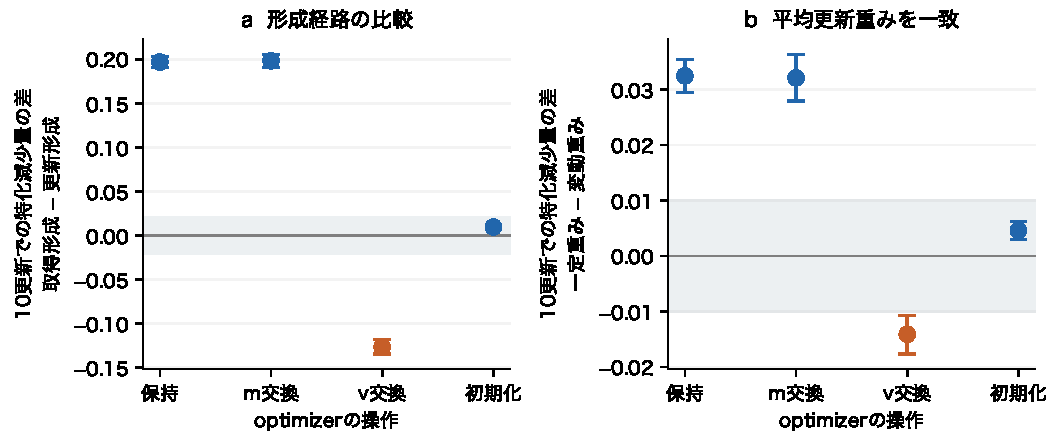
\includegraphics[width=.88\textwidth]{../figures/moments_ja.pdf}
\caption{二次モーメント交換は、二つの短時間応答対比を逆転させる。(a) 取得形成から更新形成を引いた特化低下量。(b) 取得と平均損失重みを固定した、一定から変動の重み履歴を引いた対比。帯は各事前同等性幅（$\pm0.02$、$\pm0.01$）を示す。区間は対応seedブートストラップで、各比較は重複しない40確認seedを用いる。}
\label{fig:moments}
\end{figure}

\subsection{実際のパラメータ移動が倍率と応答を結びつける}
% P:mechanism6
適応倍率は、パルス中の移動とどう関係するだろうか。固定済みの追試軌道を探索的に解析し、各更新でパラメータ空間を移動した距離（ユークリッドノルム）を足し合わせて累積経路長を測る。引継ぎAdamの10更新では、取得形成／更新形成比は、累積勾配ノルムで0.987（$[0.978,0.996]$）、パラメータ経路長で1.872（$[1.844,1.902]$）である。したがって、勾配ノルムの比が1に近くても、取得形成経路ではパラメータの移動が大きい。

% P:mechanism7
同じ40 seedにおいて、経路間の経路長差と再配分応答差の相関は0.806である。一つのseedを順に評価用として除き、残る39 seedで一変数の線形モデルを当てはめると、介入前の$\bar a_v$比を使う場合は平均二乗誤差が28\%、実測経路長差を使う場合は62\%減る。基準は、残る39 seedの応答差の平均を評価用seedの値とする予測である。したがって、この探索的比較では、実際の移動を使う方が応答差をより小さな誤差で再構成できる。

% P:mechanism8
保存済み追試の40 seed対応組で移動量を制御し、全体の経路長の違いだけで対比を説明できるかを確かめた。各更新で四つの提案ベクトル（二経路、元の$v$または交換後の$v$）のノルムの幾何平均を共通目標とし、各方向を保って大きさを揃える。経路対比は元の$v$で0.0303、交換後の$v$で0.0072となり、両者の対応差は0.0231だった。したがって、全体の移動量を揃えても$v$は再配分を変えた。この学習則は軌跡自体を変えるため、通常のAdamにおける媒介割合の推定にはならない（付録~\ref{app:extension}）。

% P:mechanism9
層を限定した交換では、この効果を大きく変える介入先がencoderにあることが分かった。元の対比0.1907に対し、第1層の$v$だけを交換すると0.0115、第2層だけなら0.0611、両headなら0.1911が残った。受容側の重みと他の最適化器成分は保持する。効果は加法的ではなく、対比を独立な寄与率へ分解するのでなく、応答を変える介入先を特定する結果である。

\subsection{比較のどの部分が別の設定へ移るか}
% P:generalization
固定した手続きを、新しい32 seed対応組で四設定へ適用した。基準設定、中間層幅64、tanhをReLUへ置換、独立な対象である。四設定すべてで終点の五つの許容幅を満たした。いずれも引継ぎ状態の正の対比、$v$交換による反転、共通$\bar a_v$での交換効果を示した。初期化による同等性は条件に依存し、幅64では初期化後の対比が0.0249で、その区間は0.02より上にあった。したがって、成分交換の効果は、Adamの初期化で10更新応答が同等になるという帰結よりも広い設定で再現した。付録~\ref{app:extension}には、初期化基準の未達を含む全条件を示す。

% P:generalizationbeta
$\beta_2$と形成時間を変えると、この移植可能性の条件がさらに明確になる。二つの形成時間群とも、$\beta_2$が大きいほど引継ぎ状態の対比は大きくなったが、$v$交換がすべての対比を反転するわけではなかった。共通倍率での交換効果は六設定すべてで正だった。したがって、二次モーメントの動き方は成分効果を変え、反転と初期化同等性は学習条件に依存する。

\subsection{三対象では終点を揃えた比較が成立し、実測データでは境界が現れる}
% P:vbmain
成分効果は、代替対象が一つしかないことに依存するだろうか。対称な三つのGaussian対象について取得・更新による履歴を形成し、優先対象を変える六つの順序付き方向を調べた。8パイロットseedでは適応を観測せず終点測定だけで校正し、新規40 seedで容量2と3を検証した。応答は、元の対象と移行先との二対象配分指数の低下量とし、三対象すべての誤差を保存した。両容量で八つすべての平均終点基準を満たした。$v$交換は10更新の経路対比を反転し、共通$\bar a_v$での配置交換も両容量で対比を変えた（表~\ref{tab:bridges}）。初期化後の同等性は容量2で成立したが、容量3では区間が$+0.02$をまたいで未解決だった（付録~\ref{app:threeadapt}）。

% P:vcmain
次に、一住宅の台所、居間、洗濯室で記録された温度と湿度を三対象に置き換えた\citep{candanedo2017data,candanedo2017dataset}。雑音で観測精度を操作し、共有表現から記録値を再構成する。時間順の別区間で、学習、パイロットの読み出し当てはめ・評価、確認の読み出し当てはめ・評価を分離した。8パイロットseedで部屋ごとに校正しても終点は揃わず、新規40 seedの確認でも両容量で未達だった。一方、交換時に受容側重みを固定して$v$を変えると、共通の平均逆倍率でも応答対比が変わった。交換後の対比は容量2で負、容量3ではゼロ付近で未解決だった。したがって、実測センサ値における成分効果は確認できたが、自然データで終点を揃えた実証は残る（付録~\ref{app:natural}）。

\begin{table}[t]
\centering\small
\caption{三対象課題をまたぐ10更新応答。値は取得形成から更新形成を引いた応答対比。末列だけは共通$\bar a_v$での自己配置から交換配置を引いた対比差である。データセットごとに別の40 seedを用い、容量間では共有する。終点一致はGaussian課題だけで成立した。区間と未達基準は付録~\ref{app:threeadapt}--\ref{app:natural}に示す。}
\label{tab:bridges}
% P:bridgestable
\begin{tabular}{llrrr}
\toprule
課題、容量 & 終点 & 自己$v$ & 交換$v$ & 共通倍率の効果\\
\midrule
Gaussian, 2 & 一致 & 0.1945 & -0.1005 & 0.0825\\
Gaussian, 3 & 一致 & 0.4054 & -0.2193 & 0.1541\\
実測センサ, 2 & 未達 & 0.0601 & -0.0254 & 0.0103\\
実測センサ, 3 & 未達 & 0.1170 & -0.0090 & 0.0257\\
\bottomrule
\end{tabular}
\end{table}

\section{最適化器条件が経路差の現れる時期を変える}
\label{sec:time}
% P:time1
初期化直後の差が小さくても、学習の継続中に大きくなる可能性がある。そこで反対介入を、引継ぎAdam、新規Adam、モーメンタムなしSGDで500更新まで延ばす。SGDの共通学習率は、seed・対象方向ごとに、最初のバッチの引継ぎAdam更新ノルムと勾配ノルムを使って校正し、以後固定する。配分応答は校正に使わない。三つの継続はいずれも、Adamで形成した経路終点から始める。

% P:time2
引継ぎAdamの経路差は10--20更新で最大となる。新規Adamは10更新の0.0096から50更新の0.0274へ、校正SGDは10更新の0.0123から50更新の0.0433、100更新の0.0309へ変わる（図\ref{fig:timecourse}b）。50更新の新規AdamとSGDの区間は0.02より上にある。この幅は10更新検証で固定したもので、後の時点では参照に用いる。観測結果は、引き継いだAdam状態を除いた後にも経路差が遅れて現れることを示し、モデル側に残る差の関与を示すが、特定のパラメータや幾何学的な原因は同定しない。

\begin{figure}[t]
\centering
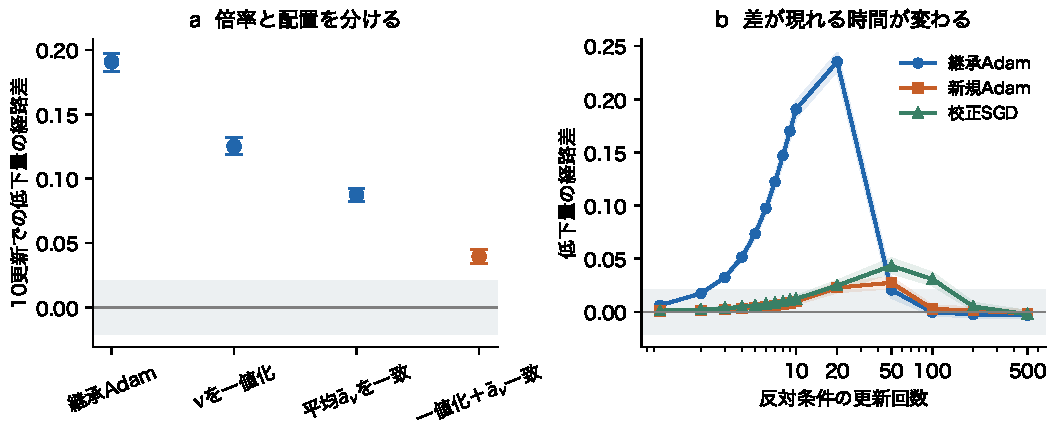
\includegraphics[width=.88\textwidth]{../figures/timecourse_ja.pdf}
\caption{倍率・配置介入と観測時間は、応答の異なる部分を明らかにする。(a) 引継ぎ状態、$v$のスカラー化、$\bar a_v$の統一、または両方の介入後の10更新経路対比。(b) 引継ぎAdam、新規Adam、校正SGDで反対条件を共通に継続する。$\pm0.02$の帯は10更新の同等性幅であり、後の時点にはこの幅による事前判定規則はない。平均と95\%対応seedブートストラップ区間は新規40 seedを用いる。}
\label{fig:timecourse}
\end{figure}

% P:time3
経路対比は500更新までにゼロへ近づく。引継ぎAdamの配分終点差は$-0.00045$（$[-0.00146,0.00057]$）である。開始測定値は近いが同一ではないため、この終点差は形成からの変化量の差とは別の量である。また、引継ぎから新規Adamを引いた応答対比は50更新までに符号を変える。そのため、新規Adamの軌道へ固定した非負の高速成分を足すだけでは、引継ぎ軌道を記述できない。この共通反対条件の範囲では、最適化器状態が再配分の時期と大きさを変え、大きな初期差が持続的な配分差を意味するわけではない。

\section{比較から得られる意義と適用範囲}
\label{sec:scope}
% P:scope1
この結果は、継続学習を検証する具体的な方法を与える。現在の特化を測り、同じ将来学習条件を加え、どの持続状態成分が応答を変えるかを調べる。本構成では、平均再構成測定値が同等でも大きな初期対比が生じ、$v$交換によって逆転する。平均的な適応倍率が説明するのは、その対比の一部である。さらに、平均損失重みを揃えた対照は、課題の平均的な重視度が同じでも、保持状態と応答が異なりうることを示す。これらの比較は、最適化器の記憶を、共有表現内の情報再配分と結びつける。

% P:scope2
具体的な応用場面は、課題を変えて学習を再開する前のチェックポイント評価である。この比較から、現在の読み出し品質に加え、最適化器状態を引き継ぐ場合と初期化する場合に、共通の継続学習を試す方法が考えられる。本実験系では、この選択によって適応の時期と大きさが変わる。同じ診断がファインチューニングの判断に役立つかは、最終的な性能を含め、対象課題で検証する必要がある。

% P:scope3
相補的な実験は、感受性を形成・維持と区別する。現在の取得は、その後の損失重みを等しくしても、1,000更新で形成済み特化を別対象へ向け直せる（\ref{app:formation}）。取得と更新を対称化すると形成済みの偏りが減り、設計した状態追従フィードバックは長く続くレジームを支えられる（\ref{app:maintenance}）。対称な三対象構成では、二つのボトルネック次元で600更新後の取得選択的形成が再現する（\ref{app:three}）。これらの対照は、形成、現在の支え、応答に異なる介入が必要であることを示す。三対象適応は、感受性についての別の検証を与える（付録~\ref{app:threeadapt}）。

% P:scope4
終点を揃えた適応の証拠は、二または三つのGaussian対象、小規模ボトルネックネットワーク、外部から指定した観測・損失重み、有限の観測時間に及ぶ。センサ拡張は一住宅の固定した時系列区間を扱い、seed区間はその記録を条件とした学習・雑音の変動を表す。終点が揃わなかったため、元の経路対比を、同等な測定に隠れた応答差へ帰属できない。自然データでこの比較を確立するには、より多様な履歴を独立に校正して終点を揃え、別の住宅や課題で検証する必要がある。座標交換は共通祖先によって定義する。全体の更新ノルムを揃えても、方向と層別の移動量は異なりうる。

\section{結論}
% P:conclusion
検証した二・三対象のGaussian系では、測定した特化が近くても追加学習への潜在的感受性が異なりうる。成分交換は、引き継いだAdamの二次モーメントが初期再配分を因果的に変えることを示した。平均適応倍率を揃えても、二対象対照では全体の更新ノルムを揃えても、効果が残った。実測センサ拡張でも成分効果は残ったが、終点一致は満たさず、介入効果の移植と隠れた応答差の実証を区別する結果となった。初期化同等性と符号反転は、容量、学習条件、観測時間に依存する。現在の読み出し品質、保持された学習状態、その後の条件が、適応の比較で現れる差をともに決める。

\section*{再現性に関する声明}
% P:repro

本稿には、匿名化したコードとデータのアーカイブを補足資料として添付する。

アーカイブには、実験I--V-CとIV-E追試およびIV-F拡張のソースコード、ローカルで固定した計画、seed別軌道、チェックポイント、監査スクリプトを含む。コードはMIT、生成データと説明資料はCC BY 4.0で提供する。再配布するUCIセンサデータは、元のCC BY 4.0の出典表示を保持する。\ref{app:status}で主張とファイルを対応づけ、CPU上での完全性・数値・図生成・学習再現の検査を示す。

\section*{広範な影響に関する声明}
% P:impact
本研究は、入力へのアクセスと学習履歴が時間とともに変わる共有表現を調べるための制御比較を提供する。運用中のシステムへ適用するには、その環境で介入と測定を直接検証する必要がある。

\section*{AI支援に関する声明}
% P:ai
生成AIシステムを、多くの実験設計と追試解析の提案、実装と実行、出力の解析、文献調査、原稿の執筆と翻訳に広く使用した。人間の著者は、研究全体を発案し、この実証研究を依頼し、主要な判断時点で継続を承認し、証拠と主張を確認し、論文とその公開について責任を負う。

\bibliography{references}
\bibliographystyle{tmlr}
\clearpage
\appendix
\section*{付録の案内}
% P:appguide
\ref{app:optimizer}は、中心となる適応比較の介入詳細と推定値を示す。\ref{app:formation}、\ref{app:maintenance}、\ref{app:three}は、それぞれ、特化がどう形成されるか、継続学習中に何がそれを支えるか、形成が三対象へどう広がるかを調べる。\ref{app:measurement}と\ref{app:calibration}は、測定の確認と取得・圧縮の校正を記す。\ref{app:coordinate}は不成立だった条件付き予測器を、\ref{app:factors}は最初の不成立と基準改訂後の検証を含む要因対照を報告する。\ref{app:status}では、それらの統計的地位を区別し、証拠と再現ファイルを対応づける。 付録~\ref{app:extension}には、終点からの予測、固定手続きの追試、移動量と層を制御した介入を示す。 付録~\ref{app:threeadapt}と\ref{app:natural}は、三Gaussian対象と実測センサ値での適応を検証する。

\section{終点と最適化器の対比（IV-D--E）}
\label{app:optimizer}
% P:appopt1
IV-Dでは40確認seedと、seedごとの二つの鏡像方向を用いる。符号を揃えた平均$s$は、取得主導形成で0.3375、更新主導形成で0.3439である。対応する対象側・非対象側誤差は0.4034/0.8144と0.4000/0.8198である。経路強度はパイロットで校正しており、確認終点へ当てはめていない。中立継続の積分差は、Adam引継ぎで$-0.0025$（$[-0.0064,0.0013]$）、初期化後で$-0.0018$（$[-0.0068,0.0030]$）である。取得、更新、複合パルスにおける引継ぎと初期化の応答交互作用は0.1657、0.1390、0.1848であり、いずれも事前基準0.08を上回る。

% P:appmargins
形成の許容幅は、符号を揃えた$s$、対象・非対象誤差とその和で$\pm0.02$、低精度の符号を揃えた$s$で$\pm0.01$である。IV-Dは、応答の判定幅として、中立継続と初期化後応答に$\pm0.02$、引継ぎ状態のパルスに$\pm0.05$を用いる。IV-Eは$m$交換による変化と初期化後応答に$\pm0.02$、経路内の更新履歴対照は初期化後応答に$\pm0.01$を用いる。これらの基準を、対応差の平均の区間へ適用する。

% P:appmarginrule
IV-Dでは、95\%区間全体が指定幅の内側に入れば同等、正負いずれかの境界の外側に完全に出れば実質差あり、それ以外は未解決と判定する。引継ぎ条件の三つのパルス区間は、いずれも全体が$+0.05$より上にあり（表\ref{tab:pulses}）、正の実質的な経路差を示す。初期化条件の全パルス区間は$\pm0.02$内に入る。

% P:appmarginorigin
IV-Dはパイロットseed 8000--8015で経路強度を校正し、seed 8100--8139の前に許容幅を固定する。IV-Eはパイロットseed 9000--9015を用いて応答基準を定め、その後にseed 9100--9139を実行する。経路内対照は、パイロットseed 9200--9215を応答基準と同等幅の設定に明示的に用い、その後にseed 9300--9339を実行する。計画にはこれらの操作上の選択が記録されているが、独立した実用誤差の基準から許容幅を導いてはいない。したがって、同等性は、これらの人工的な比較で明示した分解能における一致を表す。

\begin{table}[h]
\centering\small
\caption{成分介入下の複合パルス応答差。IV-Eは取得形成から更新形成を引いた比較、対照は一定から変動の更新重み履歴を引いた比較である。それぞれ重複しない40確認seedを用いる。}
\label{tab:components}
\begin{tabular}{lcc}
\toprule
成分条件 & IV-E経路差 & 平均を揃えた更新履歴対照\\
\midrule
自己の状態 & $0.1968\ [0.1910,0.2029]$ & $0.0324\ [0.0294,0.0354]$\\
$m$交換 & $0.1982\ [0.1912,0.2054]$ & $0.0321\ [0.0277,0.0362]$\\
$v$交換 & $-0.1265\ [-0.1348,-0.1183]$ & $-0.0141\ [-0.0176,-0.0110]$\\
初期化 & $0.0097\ [0.0078,0.0117]$ & $0.0046\ [0.0031,0.0062]$\\
\bottomrule
\end{tabular}
\end{table}

% P:appopt2
IV-Eでは、自己状態から$m$交換を引いた変化は$-0.0014$（$[-0.0044,0.0018]$）で、$\pm0.02$内にある。取得形成経路の二次モーメント総量は更新形成経路の0.5577倍であり、座標別の二次モーメント逆スケーリング係数の平均は1.950倍である。この係数は実際のパラメータ更新量の比ではない。Adamの更新は、一次モーメント、現在勾配、バイアス補正にも依存する。主要成分比較を表\ref{tab:components}に示す。

% P:appopt3
平均を揃えた更新履歴対照は、500更新の対象重み平均を0.80に固定する。一定から変動を引いた終点対比は、符号を揃えた$s$が0.0023（$[-0.0024,0.0072]$）、対象誤差が$-0.0020$（$[-0.0043,0.0002]$）、非対象誤差が0.0001（$[-0.0042,0.0043]$）、総誤差が$-0.0019$（$[-0.0039,0.0002]$）、低精度の符号を揃えた$s$が0.000756（$[-0.000532,0.002110]$）である。二次モーメント比は0.8215（$[0.8140,0.8283]$）、逆スケーリング比は1.1524（$[1.1441,1.1615]$）である。事前の終点・応答基準はすべて通過する。推論対象は、重みのばらつきと実現系列を同時に変えた効果であり、順序単独の効果ではない。

% P:appopt4
事前固定追試は新規40 seed（20000--20039）を用いる。Adamの設定は$\eta=0.002$、$\beta_1=0.9$、$\beta_2=0.999$、$\epsilon=10^{-8}$、weight decay $10^{-5}$である。step countを$t$、パラメータ数を$P$とし、
\begin{equation}
\bar a_v=\frac{1}{P}\sum_{j=1}^{P}\frac{\eta}{\sqrt{v_j/(1-\beta_2^t)}+\epsilon}
\end{equation}
を定義する。取得形成／更新形成比は、$v$総量で0.5539（$[0.5350,0.5732]$）、$\bar a_v$で1.9042（$[1.8710,1.9387]$）である。これらの比はseed・対象方向ごとに計算し、seed内で方向を平均した後、seed間で平均する。$v$がパラメータ間で一様なら、総量比から予測する逆倍率比は1.3513（$[1.3282,1.3745]$）に留まる。二次モーメントを担う座標の実効的な数を要約する探索的な参加比は、それぞれ19.17と38.93である。二次モーメントの総量だけでは、実測した平均逆倍率を再現できず、座標間の不均等もその差に関係する。

共通倍率介入では、二経路の$\bar a_v$の幾何平均を目標$a_\ast$とした。配置を保つ再調整では各座標を$c v_j$へ置き換え、$\bar a_v(c)=a_\ast$となる正の$c$を二分法80反復で求めた。配置交換では、他経路の座標別$v$を受容側の対応座標へ移植した後、同じ再調整を行った。一値化では全座標を
\begin{equation}
v_j=\left(\frac{\eta}{a_\ast}-\epsilon\right)^2(1-\beta_2^t)
\end{equation}
へ置換した。受容側自身の倍率でスカラー化するときは、$a_\ast$を幾何平均ではなく、その経路自身の$\bar a_v$とする。受容側のモデル重み、一次モーメント、step countは固定し、倍率の相対誤差は$2\times10^{-6}$未満だった。座標介入は、共通checkpointから分岐したモデル間で定義した。校正SGDはmomentum 0、同じweight decayを用いる。seed・優位対象ごとに、最初の共通batchにおける引継ぎAdamの更新ノルムを正則化込み現在勾配ノルムで割り、その二経路の幾何平均を共通学習率として以後固定した。範囲は0.0194--0.0529、平均0.03545であり、配分応答は校正に用いていない。

\begin{table}[h]
\centering\small
\caption{二次モーメントの平均倍率と座標配置を事後的に再結合した探索的解析。固定済み追試CSVから計算した、反対条件10更新後の特化低下量の経路差（取得形成から更新形成を引いた値）を示す。}
\label{tab:vdecomp}
\begin{tabular}{lc}
\toprule
二次モーメント条件 & 経路差 $[95\%\ \mathrm{CI}]$\\
\midrule
経路固有の倍率と配置 & $0.1907\ [0.1835,0.1975]$\\
経路固有の倍率、一値配置 & $0.1251\ [0.1187,0.1316]$\\
共通$\bar a_v$、経路固有の配置 & $0.0875\ [0.0825,0.0925]$\\
共通$\bar a_v$、一値配置 & $0.0395\ [0.0342,0.0447]$\\
\bottomrule
\end{tabular}
\end{table}

% P:appopt5
表\ref{tab:vdecomp}の事後的$2\times2$交互作用は0.0176（$[0.0151,0.0198]$）で、対応する加算的再構成は実測平均の90.8\%に達する。これらの組合せと統計量は固定した解析計画に含まれず、独立な加算的原因を確立しない。事前固定介入では、他経路の$v$配置へ交換して$\bar a_v$を揃えると、経路差は$-0.0110$となる。旧seedで当てはめた予測器は、新seedの応答\emph{差}の予測を改善するが、応答比の予測には失敗する。$\bar a_v$比は相対的な倍率を含むが、分母側の応答の絶対水準を含まないため、両結果は矛盾しない。

% P:appopt6
反対条件を継続したとき、10、20、50、100、200、500更新の特化低下量の経路差は、引き継ぎAdamで0.1907、0.2353、0.0207、$-0.0003$、$-0.0023$、$-0.0031$、新規Adamで0.0096、0.0228、0.0274、0.0029、0.0011、$-0.0014$、校正SGDで0.0123、0.0248、0.0433、0.0309、0.0050、$-0.0022$である。50更新時点の区間は、新規Adamで$[0.0227,0.0321]$、SGDで$[0.0368,0.0499]$である。500更新時点の配分終点差は$-0.000454$（$[-0.001462,0.000568]$）であり、形成終点からの低下量差$-0.003065$（$[-0.005642,-0.000316]$）とは別の量である。10更新パルス後に中立条件へ戻す別軌跡では、配分指数の差が50更新の0.06197から510更新の0.00984へ縮小する。引継ぎAdamから新規Adamを引いた差は50更新までに符号を変えるため、新規Adamの軌道へ固定的で非負の高速成分を足すだけでは十分に記述できない。完全状態の収束は未検証である。

% P:appopt7
事後的な更新経路解析は、固定済み追試CSVだけを読む。ここでは、まず各経路・seed内で二つの対象方向を平均し、その後にseed内で経路比を求め、seed間で平均する。以下の四つの比はこの規約を共通に用い、上記の方向別に求めた比を平均する規約とは異なる。引継ぎAdamにおける取得形成／更新形成比は、$\bar a_v$が1.900（$[1.867,1.935]$）、最初のパラメータ変位が2.028（$[1.938,2.116]$）、10更新の累積パラメータ経路長が1.872（$[1.844,1.902]$）、累積勾配ノルム経路長が0.987（$[0.978,0.996]$）だった。

% P:appopt8
seed間の相関と再構成では、$\bar a_v$比は各方向の経路比をseed内で平均し、全体の平均が1.9042となる規約を用いる。一方、パラメータ経路長比は、各経路・seed内で対象方向を平均してから経路間の比を取る。倍率比とパラメータ経路長比の相関は0.797（$[0.644,0.889]$）、二経路のパラメータ経路長差と配分応答差の相関は0.806（$[0.681,0.889]$）だった。一つのseedを順に除外する線形再構成では、$\bar a_v$比によって平均二乗誤差が28\%、実測経路長差によって62\%減った。各回のモデルの当てはめと平均だけの基準は、いずれも残る39 seedを用いる。

% P:appopt9
経路長は介入中に測定し、移動方向を捨て、それ自体へ介入していない。したがって、倍率と応答を結ぶ機構の候補を記述する量であり、因果的に媒介する効果を定量化するには、実際の移動を制御する必要がある。この再構成は、これら40 seedで測定した10更新応答を評価するもので、形成終点だけからの事前予測とは異なる。


\section{形成と移行の対照（IV-A--C）}
\label{sec:controls}
\label{app:formation}
\subsection{損失重みが等しくても、入力精度が特化を選ぶ}
% P:controls1
まず、損失重みを不均等にせずに優位性が形成されるかを問う。100回の均衡した初期化更新の後、各チェックポイントを九つの形成条件へ複製する。三つの取得条件（$A$精密、均衡、$B$精密）と、三つの更新配分（$0.85/0.15$、$0.50/0.50$、$0.15/0.85$）を交差させる。形成は500更新である。均衡取得では、各対象を精密に観測する更新を正確に250回ずつ、無作為順序で含める。すべての条件で、高精度情報の総量は同じである。

% P:controls2
損失重みが等しい条件で、$A$を精密に取得すると平均$s=0.3385$、$B$を精密に取得すると$s=-0.3338$となる。対応差は0.6723（$[0.6660,0.6794]$）で、事前基準0.30を上回る。すべての確認seedで、精密に取得した対象が優位となり、均衡取得ではほぼゼロに留まる。全条件を共通入力と新たに当てはめた読み出し器で評価しているため、この差は、学習時にきれいな信号を見た瞬間の有利さを越えて残っている。この系では、明示的な更新重みが対称でも、取得精度だけで特化を選択するのに十分である。

% P:controls3
全要因の結果は、これが情報と学習の固定的な役割分担ではないことを示す（図\ref{fig:controls}a）。どちらの制御も対象を優位にできる。両者が一致すると特化が強まり、競合すると弱まる。検証した強度では、反対側への強い更新重みが取得の優位を上回ることがある。両者は同じネットワークの勾配を通じて作用するため、介入が異なっていても、その効果が直交するとは限らない。これらは500更新時点の結果であり、極限の平衡状態の推定ではない。

\subsection{取得は、すでに形成された状態も別の対象へ移行させる}
% P:controls4
取得が重要なのは、特化が形成される前だけだろうか。両対象を雑音標準偏差0.15で観測しながら、非対称な更新によって$A$優位・$B$優位のチェックポイントを形成した。その後、更新重みを$0.50/0.50$に固定し、同じ三つの取得条件を1,000更新にわたり適用した。中立なチェックポイントも追加の参照とした。

% P:controls5
反対対象の取得によって、両初期状態の全40 seedで優位対象が入れ替わる（図\ref{fig:controls}b--d）。形成済み状態について平均した、終点の$A$精密条件と$B$精密条件の差は0.7161（$[0.7108,0.7213]$）であり、中立起点の差0.7086に近い。均衡取得では、両形成済み状態が中央へ向かう。最初のゼロ交差は平均記録時刻16.9更新と16.8更新で起きるが、その後の軌道は非単調に動きうるため、これらの時刻は落ち着いた適応までの時間を測るものではない。観測した1,000更新の範囲では、後続の損失重みが等しくても、現在の取得は更新によって形成された表現を別の対象へ移行させられる。

\begin{figure}[t]
\centering
\includegraphics[width=\textwidth]{../figures/controls_\figlang.pdf}
\caption{現在の取得と更新は、特化を共同で制御する。(a) 取得と更新の九つの組合せにおける、500形成更新後の平均配分。中央列は更新重みが等しい条件である。(b--d) 後続の更新重みをすべて等しくしても、取得によって、事前に$A$優位・$B$優位へ形成した状態を移行させられる。中立な初期状態を参照として置く。曲線は1,000更新にわたるseed平均である。初期に非単調な変化があるため、最初のゼロ交差と、持続的な転換や収束を区別する。}
\label{fig:controls}
\end{figure}

\subsection{強い片側更新では、比較の意味が変わる}
% P:controls6
別の形成済み状態の実験では、更新対象を厳密に片側へ固定し、以前優位だった対象または反対対象を精密に取得する条件と交差させた。各形成済みチェックポイントを四条件へ複製し、400更新を行う。基準対象だけを更新すると159/160セルでその優位が保たれ、反対対象だけを更新すると全セルで反対対象が優位になる。しかし、反対対象の更新を固定したまま比較すると、その対象を精密に取得する方が、基準対象を精密に取得する場合より移行軌道を速める。共通の高精度プローブでは、最初のゼロ交差までの平均時間差は3.44更新（$[2.81,4.00]$）である。事前固定した手順から得た、より大きな閾値に固有の推定値とその監査は、\ref{app:measurement}に残す。

% P:controls7
終点の深さも、取得と更新の組合せに依存する。探索的解析では、取得対象と更新対象が一致する条件は、交差する条件よりも、共通プローブでの$|s|$が0.1411大きい。二つの更新対象の下で取得の条件付き効果が逆符号になるため、取得の主効果は平均するとほぼゼロになる。したがって、取得は速度だけを制御し、更新は方向だけを制御する、という一般則をデータは支持しない。取得は優位対象を選び、入れ替えることができる。十分に強い片側更新は結果を拘束するが、その場合も取得は軌道と終点の深さを変える。


\section{形成、現在の制約、フィードバック対照（II--III）}
\label{app:maintenance}
\label{sec:maintenance}
\subsection{形成条件が、そのまま持続する偏りとして残るとは限らない}
% P:maintenance1
偏りが形成された後、その持続を観測するだけでは、現在何がそれを支えているかは分からない。そこで、支えとなる条件を取り除き、あるいは変更する。非線形の二対象ネットワークで、取得精度と更新重みをともに対称化すると、共通プローブの平均$|s|$は400更新の間に約0.41から0.04へ低下する。減衰は最終観測区間まで続く。両方の制御を対称化しているため、この介入が特定するのは両者を合わせて取り除く効果であり、偏った更新だけの必要性ではない。

% P:maintenance2
別の線形ボトルネック実験では、形成中と継続学習中の条件を交差させる。制約条件は一次元表現と一対象更新を組み合わせ、非制約条件は二次元表現と両対象更新を用いる。形成時の制約を解除すると、平均$|s|$は0.9706から0.1303へ低下する。これは一度も制約しなかった基準値0.0592より大きいが、形成時の偏りを大きく下回る。追加の交差実験で容量と更新機会を区別し、その詳細を以下に示す。これらの介入は、形成履歴が残存差を残しても、現在の条件を変えた後に元の大きさを維持するとは限らないことを示す。

\subsection{状態追従フィードバックは、長く持続するレジームを支える}
% P:maintenance3
現在働く維持機構を検証するため、関連するtanhネットワークへ完全な入力を与えながら、どの対象を更新するかを設計した規則で選ぶ。強化型の規則は現在の配分指数に追従し、よりよく表現されている対象を優先的に更新する。固定傾向対照では、同じ規則の確率を初期値で固定する。探索型規則は、表現精度が低い対象を優先する。これらの介入は、学習状態を継続して追うことと、当初から一方を多く抽出する傾向を分離する。

% P:maintenance4
三つの検証は、それぞれ異なる問いに答える。第一に、外から与えた強い履歴差は、その後の共通更新でほぼ消える。第二に、明示的な履歴操作がなくても、状態追従フィードバックは偶発的な初期差を増幅する。終点$|s|$は0.8683で、固定傾向の0.4207を上回る。第三に、別の鏡像履歴実験では、状態追従と固定傾向の間で、履歴の符号付き効果には検出可能な差がないが、絶対的な特化深度には差がある。フィードバックの結果が示すのは増幅と維持であり、履歴が指定した符号を特に強く選ぶことではない。別々の比較を以下の詳細推定値に記す。

% P:maintenance5
容量は、維持される特化を変える。三次元ボトルネックでは一方の対象にほぼ排他的な読み出しの優位が生じ、二次元では、それほど極端ではない優位をそれぞれ反対の対象にもつ二つのレジームが生じる。弱い反対側更新パルスの後には復帰し、強いパルスではレジームが転換しうる。どちらの対象も外から優遇しない条件で、大部分の軌道は8,000更新の比較期間を通じて初期のレジームを保持する。この有限時間での滞在、復帰、転換、共存を、操作的に「準安定」と呼ぶ。維持数、長時間観測、ヒステリシス検証は以下に記す。この証拠は、永続する双安定性を確立するものではない。

% P:maintenance6
非対称な定常状態には\citet{harris1997ocular}という古典的な先例があり、\citet{kiselev2026bifurcation}は正のフィードバックに基づく近年の最小分岐構成を示している。発達における形成と維持も以前から区別されている\citep{crair1998visual}。本研究の貢献は、学習された共有表現において、これらを介入により実現し比較することである。特化の持続を履歴だけに帰属させるのでなく、それを維持する現在の条件を実験で特定する。


\subsection{詳細な推定値}
% P:appmaint1
実験IIは、隠れ幅24のtanhエンコーダと線形ヘッドを用い、パラメータ数は$d_Z=2$で236、$d_Z=3$で267である。ミニバッチごとに一対象を更新する。主要な強化則は$p_A(s_t)=0.5+\alpha\tanh(\beta s_t)$であり、$\alpha=0.40$、$\beta=1.5$とする。探索では加算を減算へ変える。均衡更新は$p_A=0.5$、初期固定更新は$p_A(s_0)$を固定する。

% P:appmaint2
履歴除去、履歴を与えないフィードバック、鏡像履歴の検証は別々である。第一の検証では、強く与えた履歴差が、その後の共通学習で1.8822から0.0047へ低下する（残存比0.002）。弱い共通偏りでは比0.003となる。第二の確認seed 300--339では、初期履歴を与えない。終点$|s|$は、均衡0.1817、固定0.4207、状態追従0.8683、探索0.0580である。状態追従と固定の比は2.064で、対応のある絶対値差の区間は$[0.368,0.527]$である。

% P:appmaint3
第三の検証では、最初の100更新に、現在状態と独立な55:45と45:55の鏡像系列を用いる。この探索的比較では重複しない二組の40 seedを合わせ、直後の符号付き効果は0.0811である。終点の符号付き効果は、固定0.2240、状態追従0.2170、探索0.0015であり、最初の二つは区別できない。絶対偏差は0.4503と0.8736で、比1.94、対応差0.4233（$[0.3873,0.4596]$）となる。鏡像50:50順序対照はゼロと整合する。これらの比較は、状態追従へより強い符号付き履歴効果を帰属させずに、深さへの効果を支持する。

% P:appmaint4
容量とレジームの検証では、終点$|s|$が$d_Z=3$で0.9842、$d_Z=2$で0.3902（$[0.3790,0.4015]$）となる。80鏡像群の97.5\%が枝の大きさの中央値から25\%以内に入り、各符号に48.7\%ずつ分布する。別の長時間実行では、8,000から16,000更新の間の$|s|$変化が$-0.0004$（$[-0.0141,0.0134]$）となる。8,000形成更新後、$K=0,800,1600,3200$の反対対象強制を与えると、転換確率は$0,0.20,0.425,0.65$である。復帰・転換軌道は、対応する元の側・反対側の大きさの0.985倍、1.015倍に達する。

% P:appmaint5
外部更新偏り$h=0$で、正側と負側の準備状態は8,000更新の間に39/40、40/40でレジームを維持する。強制しない転換が一例観測される。偏り掃引の全40 seedで転換と復帰が起こり、平均閾値間隔は0.1237（$[0.1144,0.1337]$）となる。診断用10 seedでは、各偏り水準500更新での間隔0.2150が、2,000更新で0.1575、8,000更新で0.1150へ低下する。滞在、復帰、転換、共通条件下の共存が、操作的な準安定性の主張を定める。滞在時間による傾向があるため、準静的ヒステリシス幅が非ゼロだとは推論できない。

% P:appmaint6
IIIの線形制約解除実験は、独立な対象信号を用いる。$U$は二次元・両対象更新、$C$は一次元・一対象更新を表し、第一文字が形成、第二文字が測定期の継続学習を示す。終点$|s|$はUCで0.9862、CCで0.9856である。CUは形成時0.9706から0.1303へ低下し、UUは0.0592である。二つの制御をさらに分けると、一次元・両対象更新で0.9037、二次元・一対象更新で0.3368となる。この構成はIVの相関をもつ非線形ネットワークとは異なり、同じ要因実験の追加セルではなく、相補的な制約介入を提供する。


\section{三対象形成の推定値（V-A）}
\label{app:three}
\label{sec:three}
% P:three1
二対象では、すべての相対変化が一つの比較軸上にある。そこで、対ごとの相関が0.35の、対称な三つの三次元ガウス対象を九次元入力へ混合し、形成結果を検証する。エンコーダは隠れ幅32、ボトルネック次元は二または三である。更新重みは$1/3$に保つ。600更新を通じて$A$、$B$、$C$のいずれかを精密に取得し、均衡取得では各対象へ正確に200回ずつ精密観測を割り当てる。各seedでは同じ初期化済み状態から分岐する。三次元ボトルネックは、二対象系の圧縮率に一致すると同時に、一対象の次元にも等しいため、圧縮率だけを揃える純粋な対照ではない。

% P:three2
形成後にエンコーダを固定する。未使用のプローブ標本で新たな線形読み出し器を当てはめ、別の未使用標本に共通の高精度入力を与えて評価する。相対誤差を、中心化した対数誤差得点で要約する。
\begin{equation}
q_i=\frac{1}{3}\sum_{j\in\{A,B,C\}}\log D_j-\log D_i,\qquad \sum_i q_i=0.
\label{eq:q}
\end{equation}
正の得点は、誤差の幾何平均より精密に読み出せることを示す。この観測可能な配分平面は二つの座標で記述できる。それらは内部表現全体の座標ではなく、その大きさを二対象の指数$s$と直接比較することもできない。

% P:three3
両ボトルネック次元において、すべての対象別取得条件で、指定対象が全40確認seedで優位になる。均衡取得と比較した指定対象の配分得点の利得は、二次元ボトルネックで約0.37、三次元で0.90--0.92である。介入効果は配分平面上にも広がる（図\ref{fig:three}）。この広がりが一つの経験的な比較軸で説明できるかを調べるため、三つの平均介入効果ベクトルを特異値で要約する。第二特異値は、最もよく当てはまる一本の軸だけでは表せない成分を測る。その値は二つの容量でそれぞれ約0.55と1.37であり、区間はゼロを含まない。第二特異値と第一特異値の比が1に近いことは、さらに、意図したラベル対称性を確認する。正確な推定値と区間は以下に示す。また、精密取得では均衡取得より総再構成誤差が増える。この結果は読み出せる情報の再配分であり、全対象の一様な改善ではない。

\begin{figure}[t]
\centering
\includegraphics[width=\textwidth]{../figures/three_targets_\figlang.pdf}
\caption{三対象の取得効果は、観測可能な配分平面上に広がる。各点は、更新重みをすべて等しくしたときの、各seedの対象別取得効果を、そのseedの均衡取得条件との差として示す。矢印はゼロと平均を結んで終点効果を要約し、軌道は示していない。座標は$q_A$と$q_B$の利得であり、和がゼロであることから$q_C$の変化が決まる。両ボトルネック次元で、ラベル対称かつ一直線上にない三つの効果が見られる。}
\label{fig:three}
\end{figure}

% P:three4
この実験は、取得による形成の選択を三対象へ広げ、第二の観測可能な比較方向を確認する。付録~\ref{app:threeadapt}では、その後の適応と成分交換を検証する。三つの形成状態が共通条件で持続するかは、別の維持介入で調べる必要がある。


\subsection{詳細な推定値}
% P:appthree1
V-Aでは40確認seedを用い、両容量で各seedを条件間に複製する。高精度取得利得は、指定対象の中心化対数誤差得点の、均衡取得に対する変化である。更新の陽性対照は、均衡取得で重み$0.8/0.1/0.1$を用いる。表\ref{tab:three}に対象ラベル間の範囲を示す。すべての対象別取得条件で、全seedの指定対象が優位となる。

\begin{table}[h]
\centering\small
\caption{600更新後の三対象形成。利得と総誤差の範囲は三つの対象ラベルにわたる。特異値は対象別介入効果行列を要約し、報告値はブートストラップ平均である。}
\label{tab:three}
\begin{tabular}{ccccc}
\toprule
$d_Z$ & 取得利得 & 更新対照利得 & $\sigma_2$ & 総誤差増加\\
\midrule
2 & 0.3701--0.3731 & 0.4635--0.4668 & 0.5535 & 0.0749--0.0767\\
3 & 0.9030--0.9232 & 1.2239--1.2297 & 1.3656 & 0.1138--0.1148\\
\bottomrule
\end{tabular}
\end{table}

% P:appthree2
$\sigma_2$の区間は、$d_Z=2$で$[0.5456,0.5612]$、$d_Z=3$で$[1.3491,1.3815]$である。比$\sigma_2/\sigma_1$は0.9839（$[0.9725,0.9947]$）、0.9876（$[0.9767,0.9971]$）で、事前基準0.70を上回る。第二対比が非ゼロであることと、ほぼラベル対称であることは異なる主張であり、どちらも内部学習状態の次元を特定しない。最良線形符号の歪み床（0.3344と0.0025）に対する探索的正規化では、取得によって除去可能な歪みの63.23\%、63.67\%が除かれ、更新対照では75.61\%、75.39\%が除かれる。これらの類似は、容量不変性の確認的検証を構成しない。 共通低精度プローブでも、対象とseedを平均した指定対象の配分得点は容量2で約0.137、容量3で約0.235と正だった。


\section{ネットワーク、取得、測定の詳細（IV）}
\label{app:measurement}
% P:appmeasure1
中心となるIVネットワークは$6\to32\to2$構造をもち、エンコーダ各層の後にtanh、その後に線形再構成ヘッドを置く。IV-Bの訓練・プローブ・テスト標本数は3,072/768/1,536、バッチサイズ256、学習率0.002、重み減衰$10^{-5}$、事後読み出しのリッジ係数$10^{-3}$である。雑音を含む対象チャネルは、直交混合の前に$\sqrt{1+\sigma^2}$で除す。訓練対象には雑音がない。IV-Bでは100初期化更新と500形成更新を用い、IV-Cでは形成済み状態から1,000更新を続ける。訓練ヘッドと事後読み出しヘッドは線形でも、これらのモデルは非線形共有エンコーダである。

% P:appmeasure2
IV-Aは、40 seedの二つの鏡像形成状態を、四つの取得・更新セルで400更新追跡する。元のプローブでは、反対対象更新を固定したとき、事前指定の符号を揃えた閾値$-0.08$に達する時間が、基準側取得で40.6更新、反対側取得で22.2更新となる。差は18.4（$[13.2,25.8]$）である。保存された軌道を共通低雑音入力で再測定すると、配分範囲は約$[-0.154,0.160]$から$[-0.451,0.462]$へ広がる。元入力の監査行は元軌道とビット単位で一致する。新しい学習実行でなく、測定の追加である。

% P:appmeasure3
最初のゼロ交差の差は、元プローブで3.50、共通プローブで3.44（$[2.81,4.00]$）である。元の閾値を0.04、0.06、0.08へ変えると、時間差は6.50、8.44、18.38へ変わる。0.10以上の閾値では未到達が増え、右打切りの影響を受けやすくなる。したがって事前指定の18.4は閾値に固有の推定値であり、ゼロ交差と連続軌道の効果が一致することが、測定をまたいだ取得効果の向きを支持する。

% P:appmeasure4
探索的な終点深度の整合対比は、元プローブで0.0376、共通プローブで0.1411（$[0.1370,0.1455]$）である。共通プローブの取得主効果は0.0002（$[-0.0011,0.0014]$）であり、条件付き効果は基準対象更新で$+0.1413$、反対対象更新で$-0.1410$と逆符号になる。取得・更新の対称継続では、元プローブの$|s|$は0.1326から0.0146、共通プローブでは0.4067から0.0413へ低下し、平均残存比は0.1009である。これらの結果は、終点深度、軌道、維持を、すべて取得主効果へ帰属させずに区別する。

% P:appmeasure5
IV-Bの共通低精度プローブでも、取得対比は0.2237残る。IV-Cでは0.2344（$[0.2322,0.2365]$）であり、形成済み起点の共通高精度対比は0.7161である。これらの測定間の一致は優位対象の比較を支持すると同時に、配分指数の大きさを、測定に依存しない物理量として扱うべきでないことを示す。


\section{取得と圧縮の校正（実験I）}
\label{app:calibration}
% P:appcal1
取得の制御を、観測損失と圧縮損失を区別できる線形ガウス系で校正する。この分解は間接情報源符号化に従う\citep{shannon1959coding,wolf1970transmission}。二乗誤差の下で、対象$X$、取得データ$Y$、予測器$g(Y)$について、条件付き期待値の直交性から次を得る。
\begin{equation}
\mathbb E\|X-g(Y)\|^2=\mathbb E\|X-\mathbb E[X\mid Y]\|^2+
\mathbb E\|\mathbb E[X\mid Y]-g(Y)\|^2.
\end{equation}
同じ$Y$から作る符号を拡張するだけでは、第一項は減らせない。表現制約は第二項をさらに増やしうる。

% P:appcal2
seedごとのランダム直交変換で混合した、相関する二つの三次元対象について、観測予算$B_{\mathrm{obs}}\in\{2,3,4,6\}$でチャネル部分集合を列挙し、$d_Z\in\{1,\ldots,6\}$の最適な階数$d_Z$線形表現を当てはめる。20 seedを用い、seedごとの訓練標本数は8,192、テスト標本数は4,096である。無制約の平均歪みは0.0004であり、取得だけ、表現だけを制約すると、それぞれ0.3956、0.3262増加する。これらは取得・表現の格子状比較から得た校正対比である。二つの対象重みの下で最適な二チャネル部分集合を比較すると、Jaccard重なりの平均は0.0167であり、無作為部分集合では0.2444である。これは課題依存の取得に対する操作確認であり、混合後の対象ラベルによって必然的に決まる恒等関係ではない。

% P:appcal3
別の解析的確認では、階数三のエンコーダを用いる。このとき均衡した母集団誤差は$D_A=D_B=(1-\rho)/2$である。六つの相関値で、最適読み出しを伴う勾配学習は、この曲線にRMSE 0.0030、最大誤差0.0042で一致する。この別の校正において、三次元から六次元へ拡張すると歪みは0.3236改善する。格子状比較の差0.3262とは別の値である。

% P:appcal4
逐次検証では、各回に$A$または$B$を見る四回の観測を与え、16通りの固定系列を作る。雑音を含む初期手掛かりが、その後に重要になる対象を予測する。手掛かり依存方策は、内部の学習済み状態を繰り返し追うのでなく、一度だけ完全な観測系列を選ぶ。選択には訓練30,000、検証10,000標本を用い、その後に独立なテスト20,000標本を用いる。最良の固定方策の目的値は0.181864、手掛かり依存方策は0.124223で、31.7\%低下する。同じ方策クラスで手掛かりをシャッフルすると0.181039となる。したがって利得は、クラスが大きいことだけでなく、手掛かり情報に依存する。

% P:appcal5
時間依存性は、近隣の観測系列も結合する。$L_s(W)$と$L_t(W)$を両端の方策の損失とすると、共有デコーダの超過損失
\begin{equation}
B(\alpha)=\min_W\{(1-\alpha)L_s(W)+\alpha L_t(W)\}
 -(1-\alpha)\min_W L_s(W)-\alpha\min_W L_t(W)
\end{equation}
は、$0\leq\alpha\leq1$において構成上非負である。内部の混合比で最小値が達成されるなら、超過ゼロには共通の最小化デコーダが必要となる。測定したのは、この共通最適条件が成立しなくなる頻度である。正の超過は、時間相関$\phi=0$で近隣経路0/32、0.4で4/32、0.8で18/32に生じる。最大は0.039801であり、専用デコーダを用いると超過は消える。$\phi=0.8$では、厳密な母集団方策目的に二つの局所最適があり、共同学習した13/20 seedがオラクル系列に達する。


\section{座標候補は条件付き予測に失敗する（III）}
\label{app:coordinate}
% P:appcoord1
別の検証では、ゆっくり変わる変数から、維持される特化の間の転換を予測できるかを問う。外部から指定した循環によって、表現、課題の重点を定める枠組み変数$\kappa_t$、評価感度を結合する。80群が、平均$|s|=0.9854$の履歴に整合したレジームを形成する。無摂動の8,000更新で自発的転換はなく、弱摂動からの復帰時間の90パーセンタイルは200更新であるため、観測された時間尺度比の下限は40となる。独立再確認では、反対対象への強制を$K=0,1600,3200,4000,4800,5600,6400$更新続けたときの丸めた転換確率が$0,0,0.138,0.450,0.688,0.838,0.938$となる。

% P:appcoord2
これと重複しない元の座標監査標本では、$K=4000,4800,5600$の率は0.4625、0.6250、0.8750である。AUCは、転換する軌道を転換しない軌道より上位に並べる予測能力を測る。プールした$\kappa$のAUCは0.712で、$s$の0.600を上回る。各介入水準内では、$\kappa$のAUCは0.565、0.567、0.380となる。seedを分離した五分割検証で、$K$と$s$に$\kappa$を加えたAUC変化は0.0049であり、対数損失はわずかに悪化する。したがって二組の転換率は異なる標本を記述しており、一つのCSVから得た矛盾する推定値ではない。先行するIIのヘッド間距離候補も、独立した条件付き検証に失敗する（$K=1600$でAUC 0.373）。これらは検証した予測器の不成立であり、コンパクトな動力学的座標が存在しないことの証明ではない。


\section{補助的な有限状態要因対照（III）}
\label{app:factors}
% P:appfactors1
別の資源管理環境では、課題枠組み、因果予測、予測地平、評価地平、リスク感度、停止を区別して操作できるかを調べる。制御器は、将来の故障を防ぐために設備を保守しながら、五水準の資源から現在需要へ供給する。資源水準、二値の需要、二値の設備状態により、20の外部状態を構成する。標準センサの精度は0.62、追加の対象別センサの精度は0.94である。10段先までの動的計画法オラクルが、トレードオフ環境と共通最適をもつ帰無環境について、方策とPareto参照を与える。

% P:appfactors2
最初の確認実験では、枠組みと予測地平の確認は通過するが、因果モデル、評価地平、リスク感度の基準は通過しない。遷移への介入が小さすぎ、評価効果は閾値に届かず、リスク閾値は基準リスクを上回っていた。新たな40 seedの前に、強度と到達可能な相対基準を改定して固定すると、五系列すべてが通過する。この後の成功は、最初の不成立を変更しない。枠組み変更の要因実験では、設計した規則の下で、長い予測、長い評価、枠組み可塑性が揃った場合にのみ切替が生じる。代替情報を改善すると、単に切替回数が増えるのでなく、枠組みと設備状態の一致が改善する。これらの対照は、指定した各要因を区別して操作する介入基盤を支える。


\section{統計的地位と出典対応}
\label{app:status}
% P:appstatus1
確認的結果は、事前の観測時間、対比、許容幅を保持する。IV-Aの終点深度整合性と、V-Aの除去可能歪みによる正規化は探索的である。閾値感度と条件付き予測器の検証は監査であり、主要結果を事後的に再定義する置換ではない。seed内の対応を保ち、鏡像ラベルを独立seedとしない。最初に不成立だった要因確認と条件付き予測器は、\ref{app:factors}と\ref{app:coordinate}に残す。

% P:appstatus2
問いに沿った各節は、再現記録と次のように対応する。形成と移行はIV-B、IV-C、IV-A、現在の支えはII、IIIの制約解除構成、IV-Aの中立継続、潜在的感受性はIV-D、IV-E、IV-E更新重み対照、IV-E追試、条件付き座標監査はIII-C、三対象形成はV-Aを用いる。実験Iは取得と圧縮の校正を担う。追試の事前固定介入と、後から加えた探索的再結合は別の記録に保存し、証拠地位を分ける。各構成は、それぞれに指定したパラメータの下で相補的な検証を行う。

% P:appstatus3
アーカイブ内の\texttt{docs/PAPER\_TO\_DATA.md}は、各図と主要な表を入力ファイルへ結びつける。アーカイブ直下で\texttt{python scripts/verify\_data.py}を実行すると、保存ファイルのハッシュと追試の固定済み計画・結果を照合できる。\texttt{python scripts/check\_core\_results.py}は、保存CSVから中心的な27平均値を独立に再計算する。\texttt{requirements-analysis.txt}を導入して\texttt{python scripts/make\_figures.py}を実行すると、英語図5種類を再生成できる。数値検査の対象は選択した平均値である。別の区間照合表は、印刷したすべての信頼区間を、保存結果と丸め桁数へ対応づける。鏡像履歴を合算した深さの対比とIV-Aの二つの終点深さ対比では、鏡像ラベルをseed内平均した後、対応を保つseedブートストラップを20,000回行う。これらの探索的計算は\texttt{scripts/audit\_manuscript\_intervals.py}で再現でき、事前指定の実験結果と判定基準は別に識別できる。

% P:appstatus4
学習の再実行は\texttt{docs/REPRODUCING.md}に示し、1 seedの軌道照合と40 seed全体の追試を含む。記録された追試環境は、Python 3.11.7、NumPy 2.4.6、PyTorch 2.13.0、CPU、1スレッドである。これとは別に行ったパッケージ検査の環境と範囲は\texttt{provenance/validation.json}に記録されており、過去の全実験を再実行した検証ではない。再実行の出力先を新しいフォルダにすることで、確認的データ、不成立の判定、探索的記録を比較用に保持する。 拡張部分の検証は、\texttt{provenance/ivf\_validation.json}、\texttt{provenance/vbc\_validation.json}、\texttt{provenance/head\_validation.json}、\texttt{provenance/formation\_validation.json}へ別に記録する。

% P:appfprovenance
IV-Fは\texttt{experiments/iv-extension/}に収録し、二つの固定記録にローカルでの実行前ハッシュを記す。\texttt{README.md}は、全モード、予測、層別集計、未達基準をデータと再実行手順へ対応づける。\texttt{audit\_extension.py}は、生CSVの平均、完全性、共通開始値、ノルム制約、固定ハッシュを独立に検査する。新規学習の前に、基準checkpointと六つのパルスモードが保存済みseed 20000を完全に再現した。

\section{終点予測・別設定への移植・機構の追加検証（IV-F）}
\label{app:extension}
% P:appfintro
短期応答差のどの部分が保存終点から予測でき、別のネットワークや対象へ移り、移動量を制御しても残るかを調べた。既存データ解析は重複しない三つの40 seed集合を用いる。新規学習は、未使用の同じ32 seed（32000--32031）を九設定で用いる。四つのモデル・対象設定と、二次モーメント減衰率・形成時間の$3\times2$設定で、基準設定一つを共用する。層別・移動量介入は追試の保存済み40 seed対応組を再利用する。新規実行前に計画とコードをローカル固定し、既存データ解析は探索的とする。鏡像方向はseed内平均する。区間は5,000回のseed対応bootstrapによる個別95\%区間である。

\subsection{残った終点差は応答を予測するか}
% P:appfpred
各集合で、複合パルスの応答対比を、標的誤差、他方誤差、低精度の符号整合$s$の終点対応差から予測する。最小二乗回帰では学習用標本だけで標準化し、除外したseedで評価する。基準は他の39 seedの平均を予測する。誤差比が一付近または一以上なら、予測の改善は乏しい（表~\ref{tab:ivfendpoint}）。IV-Dの係数を変更せずIV-Eと追試へ適用した誤差比は、IV-D平均の予測に対して1.032と0.999だった。切片は三つの測定特徴の差がゼロの場合の対比を推定するが、条件付きの線形記述であり、測定していない幾何を因果的に調整した値ではない。

\begin{table}[ht]
\centering\small
\caption{終点予測の探索的解析。MSE比は未使用seedの誤差を学習平均の基準と比較する。末列は条件付き切片とseed-bootstrap区間。}
\label{tab:ivfendpoint}
% P:appfendpointtable
\begin{tabular}{lrr}
\toprule
集合 & MSE比 & 終点差ゼロでの対比\\
\midrule
IV-D & 1.118 & $0.1935\;[0.1841,0.2023]$ \\
IV-E & 1.023 & $0.2001\;[0.1915,0.2081]$ \\
IV-E追試 & 0.984 & $0.1874\;[0.1776,0.1965]$ \\
\bottomrule
\end{tabular}

\end{table}

\subsection{形成手続きを変えない移植}
% P:appfgeneral1
四設定は、三次元の二対象、二次元ボトルネック、初期100更新、形成500更新、更新経路の標的損失重み0.80、共通の10更新パルスを維持する。幅64は中間層幅だけを変え、ReLUはencoderの二つのtanhを置換し、$\rho=0$は対象間の相関を除く。応答に応じた再校正は行わない。全設定で元の五つの終点許容幅を満たした。元状態、$m$交換、$v$交換、初期化、共通$\bar a_v$、共通$\bar a_v$での$v$交換を全設定で評価した。

% P:appfgeneral2
表~\ref{tab:ivfgeneral}では、全設定で引継ぎ状態の対比が正で、$v$交換後に反転した。共通$\bar a_v$での対応交換効果は、基準、幅64、ReLU、独立対象の順に0.1028、0.1568、0.0491、0.0137で、全区間がゼロより上にあった。幅64の初期化区間は0.02より完全に上にあり、固定した同等性基準を満たさなかった。したがって、成分効果はこれらの変更を越えて再現したが、初期化による同等性は全設定へ移らなかった。

\begin{table}[ht]
\centering\small
\caption{同じ新規32 seedによる固定手続きの追試。全設定で終点一致を満たす。値は10更新の経路対比と対応95\%区間。}
\label{tab:ivfgeneral}
% P:appfgeneraltable
\begin{tabular}{lrrr}
\toprule
設定 & 元の状態 & $v$交換 & 初期化\\
\midrule
基準 & $0.1962\;[0.1881,0.2043]$ & $-0.1290\;[-0.1379,-0.1198]$ & $0.0073\;[0.0054,0.0092]$ \\
幅64 & $0.2877\;[0.2788,0.2962]$ & $-0.1502\;[-0.1606,-0.1395]$ & $0.0249\;[0.0217,0.0282]$ \\
ReLU & $0.0879\;[0.0739,0.1003]$ & $-0.0831\;[-0.0921,-0.0731]$ & $-0.0026\;[-0.0045,-0.0010]$ \\
$\rho=0$ & $0.0668\;[0.0571,0.0770]$ & $-0.0901\;[-0.1001,-0.0801]$ & $0.0056\;[0.0020,0.0097]$ \\
\bottomrule
\end{tabular}

\end{table}

\subsection{二次モーメントの減衰と形成時間}
% P:appfbeta1
$\beta_2\in\{0.9,0.99,0.999\}$と形成500または1,500更新を組み合わせ、初期化・形成・パルスで同じ減衰率を用い、Adamのバイアス補正を維持した。六設定とも終点許容幅を満たした。形成500更新では、$\beta_2$の増加に沿って元の対比が0.0298、0.1385、0.1962へ増えた。最小値は下限が0.05を超えるという固定基準を満たさなかった。交換による反転は500更新後では0.99と0.999、1,500更新後では0.999だけで生じた。共通倍率での交換効果は全条件で正だった（表~\ref{tab:ivfbeta}）。

% P:appfbeta2
初期化列は、引き継いだ最適化器状態を除去した後に残る差を示す。$\beta_2=0.9$では、形成500・1,500更新後の初期化対比は0.0373と0.1073であり、元の状態の0.0298と0.0764より大きい。1,500更新後では三つの初期化区間すべてが0.02より上にある。したがって、初期化から最適化器側とモデル側の寄与を加法的に差し引くことはできない。この格子は形成軌跡とその後の適応を同時に変えるため、記憶時間だけの効果ではなく学習条件への依存を同定する。 対応seedの探索的比較では、$\beta_2=0.9$の形成500・1,500更新における初期化から元の状態を引いた増加は、$0.0075\;[0.0059,0.0090]$と$0.0308\;[0.0282,0.0334]$だった。初期化は両モーメントと最適化器のstepを変えるため、この対比は$v$だけを分離しない。

\begin{table}[ht]
\centering\small
\caption{減衰率と形成時間の組合せ。各設定32対応seed。共通倍率での配置効果は共通$\bar a_v$での$v$交換前から交換後を引いた経路対比差。全設定で終点許容幅を満たす。}
\label{tab:ivfbeta}
% P:appfbetatable
\begin{tabular}{llcccc}
\toprule
$\beta_2$ & 形成 & 元の状態 & $v$交換 & 初期化 & \shortstack{共通倍率での\\配置効果}\\
\midrule
$0.9$ & 500 & \shortstack{$0.0298$\\$[0.0278,0.0318]$} & \shortstack{$0.0104$\\$[0.0082,0.0127]$} & \shortstack{$0.0373$\\$[0.0342,0.0406]$} & \shortstack{$0.0058$\\$[0.0053,0.0064]$} \\
$0.9$ & 1500 & \shortstack{$0.0764$\\$[0.0736,0.0794]$} & \shortstack{$0.0494$\\$[0.0462,0.0526]$} & \shortstack{$0.1073$\\$[0.1023,0.1123]$} & \shortstack{$0.0120$\\$[0.0111,0.0131]$} \\
$0.99$ & 500 & \shortstack{$0.1385$\\$[0.1329,0.1444]$} & \shortstack{$-0.0720$\\$[-0.0770,-0.0672]$} & \shortstack{$0.0174$\\$[0.0150,0.0197]$} & \shortstack{$0.0673$\\$[0.0625,0.0721]$} \\
$0.99$ & 1500 & \shortstack{$0.2859$\\$[0.2789,0.2925]$} & \shortstack{$0.0297$\\$[0.0204,0.0390]$} & \shortstack{$0.0963$\\$[0.0913,0.1014]$} & \shortstack{$0.1334$\\$[0.1204,0.1448]$} \\
$0.999$ & 500 & \shortstack{$0.1962$\\$[0.1881,0.2043]$} & \shortstack{$-0.1290$\\$[-0.1379,-0.1198]$} & \shortstack{$0.0073$\\$[0.0054,0.0092]$} & \shortstack{$0.1028$\\$[0.0947,0.1109]$} \\
$0.999$ & 1500 & \shortstack{$0.4341$\\$[0.4277,0.4408]$} & \shortstack{$-0.1279$\\$[-0.1416,-0.1139]$} & \shortstack{$0.0574$\\$[0.0529,0.0618]$} & \shortstack{$0.2528$\\$[0.2414,0.2644]$} \\
\bottomrule
\end{tabular}

\end{table}

\subsection{交換はどこに作用し、移動量を揃えても残るか}
% P:appflayer
保存済み追試checkpointでは、$v$総量と平均逆倍率は異なる分布を表した。第1 encoder層は224パラメータをもち、$v$総量の割合は取得経路で5.9\%、更新経路で13.0\%、平均逆倍率は1.130対0.591だった。両headを合わせた$v$総量は66.2\%対43.9\%を占める。それでもheadの$v$だけを交換した対比変化は0.001未満で、encoderの各層の交換は対比を大きく変えた（表~\ref{tab:ivfmechanism}）。層には重みとバイアスを含める。介入効果は加法的ではなく、総量の割合を因果的な寄与率へ変換するものではない。

% P:appfnorm
実移動量を制御するため、四分岐（二経路、元または交換した$v$）が現在状態からAdam更新を提案する。四つのEuclideanノルムの幾何平均を、そのstepの共通目標とする。各ベクトルの方向を保って大きさを揃え、$m$、$v$、stepは実際の位置の勾配から更新を続ける。目標ノルムからの最大相対差は$2\times10^{-6}$未満だった。得られた交換効果は$0.0231\;[0.0208,0.0253]$である。したがって、全体の移動量が等しくても成分効果が残る。方向と層別の移動量は異なりうる。この共同制御則は、自然な軌跡での媒介割合を同定するものではない。






\subsection{保存終点におけるhead別のencoder勾配}
\label{app:headgrad}
% P:headgraddesign
追試の全40 seed（20000--20039）、両優先対象方向、両経路の160 checkpointを用いた。重みを更新せずheadも当てはめ直さず、各学習済みheadの平均二乗再構成損失を個別に微分した。元の未使用評価分割1,536例から、seedごとに256例の復元抽出バッチを32個作り、経路間でインデックス、教師信号、入力・雑音を共通にした。主たる記述用プローブは両対象高精度とし、両対象低精度、優先対象精密、他対象精密を感度分析として保持した。先の結果を知った後、この勾配を計算する前に解析をローカルで記録した探索的分析である。

% P:headgradmethod
head・encoder層ごとに、バッチ勾配ノルムの二乗を平均して平方根を取る。方向内で取得／更新比を作り、その対数をseed内で両方向について平均する。表~\ref{tab:headgrad}は幾何平均比と、5,000回の対応seed再標本化による個別95\%区間を示す。二つのhead勾配の方向の近さを余弦で測り、$-1$は逆方向、$+1$は同方向を表す。余弦はバッチと方向をseed内で平均する。明記しない勾配には損失重みを掛けず、重み減衰も別に保存する。

\begin{table}[ht]
\centering\small
\caption{共通高精度入力での探索的終点勾配。ノルム比は取得／更新、余弦行は各経路を別々に記述する。統計単位は40対応seed。}
\label{tab:headgrad}
% P:headgradtable
\begin{tabular}{lcc}
\toprule
測定量 & encoder第1層 & encoder第2層\\
\midrule
優先headのノルム比 & $1.331\;[1.304,1.360]$ & $1.122\;[1.097,1.149]$\\
他headのノルム比 & $1.150\;[1.135,1.166]$ & $1.028\;[1.014,1.041]$\\
等重み合計のノルム比 & $0.860\;[0.840,0.880]$ & $0.736\;[0.717,0.755]$\\
勾配余弦・取得経路 & $-0.976\;[-0.979,-0.974]$ & $-0.969\;[-0.973,-0.966]$\\
勾配余弦・更新経路 & $-0.853\;[-0.866,-0.839]$ & $-0.784\;[-0.799,-0.767]$\\
\bottomrule
\end{tabular}
\end{table}

% P:headgradinterpretation
共通高精度プローブでは各headの勾配比は1を超える一方、等重みで足した勾配比は1未満だった。勾配$g_f,g_o$と重み$w_f,w_o$に対し、合計の二乗は$w_f^2\|g_f\|^2+w_o^2\|g_o\|^2+2w_fw_o\langle g_f,g_o\rangle$である。負の交差項が効くため、各headのノルムを加法的な寄与率にはできない。

% P:headgradinputs
同じプローブでも経路ごとの形成重みを用いると、合計ノルム比は1.215と0.939になった。等重み比も入力に依存し、両対象低精度では1.305/1.211、優先対象精密では0.693/0.590、他対象精密では1.208/1.122だった。優先対象精密プローブは、取得経路の形成時と同じ観測精度を終点で与える条件である。この条件の第1層余弦は取得経路$-0.940$、更新経路$-0.835$だった。両対象高精度では、両経路とも他headのRMS勾配が優先headより大きい（全バッチをまとめたノルム比は1.83と2.05）。更新経路の形成重みでは、この大きいheadの重みを下げることで合計ノルムが縮む。全条件を保持しており、合計勾配が小さいという所見はプローブと重みづけに依存する。

% P:headgradassociation
これらの終点量は、seed間の応答差と対応するだろうか。両対象高精度プローブ、第1 encoder層、保存済みの元状態による10更新応答を用いて探索的に調べた。両方向をseed内で平均した後の40 seed間相関は、取得経路の余弦で$-0.22\;[-0.53,0.19]$、更新経路の余弦で$-0.17\;[-0.60,0.37]$、等重み合成勾配のRMS取得／更新比の対数で$0.52\;[0.22,0.71]$だった。個別区間は20,000回の対応seed再標本化による。四プローブ・二層の全結果を保存した。余弦との明確な関連は確認できず、中程度の関連も排除できない。ノルム比との正の関連だけでは、現在勾配と最適化器状態の寄与を分離できない。

% P:headgradscope
これらの終点結果は、形成500更新後の二対象tanh基準系を対象とする。全バッチ値と解析的監査は\texttt{experiments/iv-head-gradients/}、終点相関は\path{experiments/iv-formation-logging/endpoint_associations/}に保持する。次の分析では実際の形成勾配を追跡する。


\subsection{元の形成履歴の中で生じる勾配の打消し}
\label{app:formationlogs}
% P:formationlogdesign
二次モーメントができる過程を観測するため、追試の全40 seed、両優先対象方向、両経路を再実行した。共通の100初期更新と、各経路の形成500更新について、観測、バッチ、損失重み、Adam設定を元のまま保った。実際の学習バッチ上で各headの勾配を記録し、その後に元と同じ最適化器更新を行った。160個すべての最終モデル状態と両モーメントが、保存済みcheckpointとビット単位で一致した。この探索的再実行は80,000更新、320,000層・時点の観測を記録し、独立な学習seedを増やしてはいない。

% P:formationlogaccount
重み付きの和の二乗を、個別の二乗項とその相互作用に分ける。形成更新$t$での重みを掛ける前のhead勾配を$g_f,g_o$、結合した重み減衰を$\lambda\theta$とすると、正則化勾配は$g_t=w_fg_f+w_og_o+\lambda\theta$である。各項へ二次モーメントの減衰を適用すると、座標ごとに次の関係になる。
\begin{equation}
v_{500}=\beta_2^{500}v_0+S+C+R+E.
\end{equation}
$S$は$w_f^2g_f^2+w_o^2g_o^2$、$C$は$2w_fw_og_fg_o$、$R$は重み減衰に関する項の蓄積で、$E$は浮動小数点の丸めを記録する。各蓄積には元の係数$(1-\beta_2)\beta_2^{500-t}$を使う。負の$C$が打消しであり、$-C/S$は個別二乗項の蓄積をどれだけ相殺したかを表す。層の比では、重みとバイアスにわたり$S$と$C$を足してから割る。比はseed内で両方向を平均し、正の経路比には対数平均を用いる。個別95\%区間は5,000回の対応seed再標本化による。

% P:formationlogresult
取得経路では形成を通じて平均的に打消しが強かった（図~\ref{fig:formationlogs}）。500更新後の$-C/S$は、第1・第2 encoder層で$0.942\;[0.939,0.945]$と$0.930\;[0.927,0.934]$であり、更新経路では$0.284\;[0.271,0.298]$と$0.252\;[0.238,0.268]$だった。最終$v$の取得／更新比は、それぞれ$0.242\;[0.230,0.255]$と$0.340\;[0.321,0.361]$だった。方向ごとの割合をseed内で平均すると、取得経路の最終$v$の約64\%と79\%は初期状態からの残存分で、更新経路では16\%と28\%だった。蓄積した個別二乗項の合計$S$の平均は、両層とも取得経路の方が大きかった。したがって、小さな最終状態には、新しく蓄積する課題勾配の強い相殺と、相当量の引継ぎ成分の両方が関わっていた。

\begin{figure}[ht]
\centering
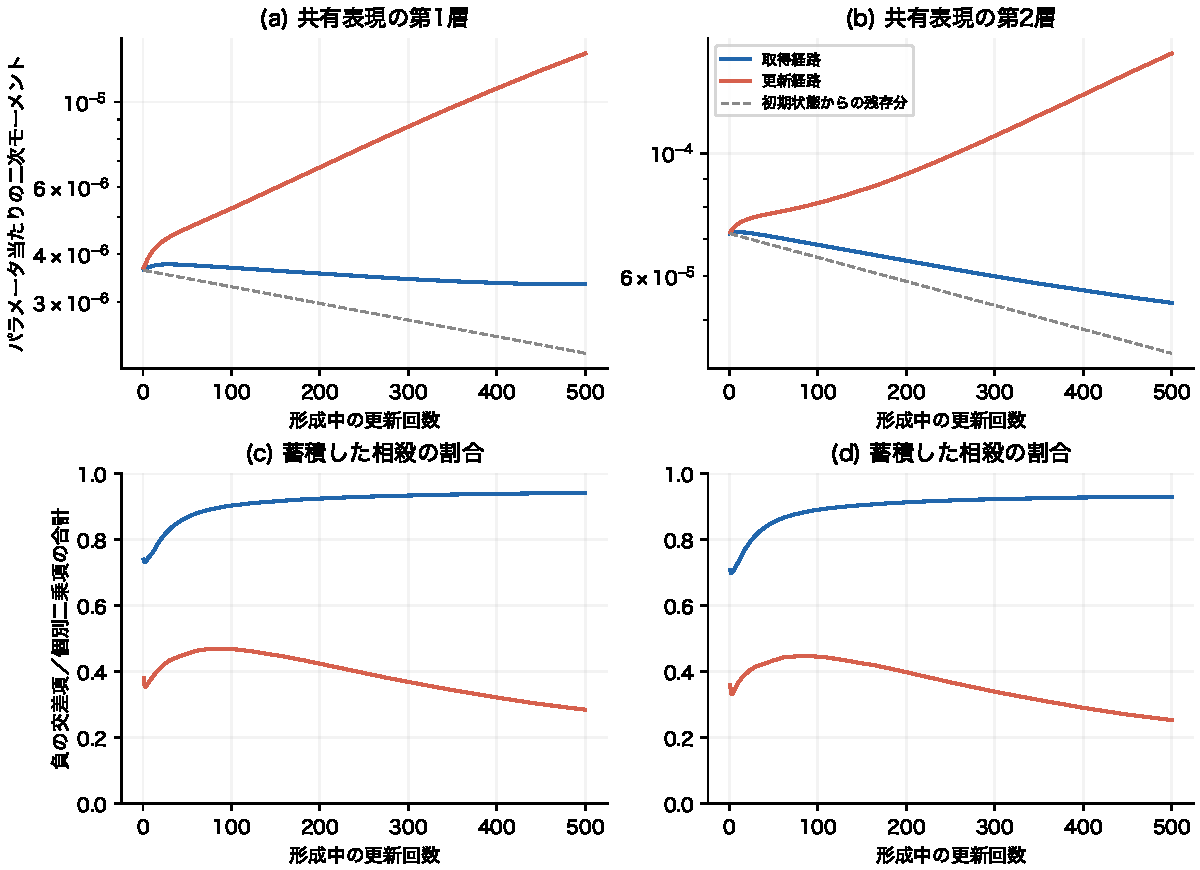
\includegraphics[width=.86\textwidth]{../figures/formation_logging_ja.pdf}
\caption{元の40対応seedによる形成中の分解。上段は各encoder層のパラメータ当たり二次モーメントの平均で、破線は共通の初期状態から減衰して残る量。下段は、各経路の実際の観測と損失重みの下で蓄積した相殺割合$-C/S$の平均。曲線は両方向をseed内で平均し、その後seed間で平均した。最終値の区間は本文に示す。}
\label{fig:formationlogs}
\end{figure}

% P:formationlogscope
この分解は、$\beta_2=0.999$、形成500更新の二対象tanh基準系を対象とする。終点プローブが入力を共通にするのに対し、実際の入力と変化する重みを追跡した。打消しを変更すれば後の重みと勾配も変わるため、その因果効果の同定には介入が必要である。解析的な連鎖律で3,840個の保存時点・層記録を独立照合し、逐次更新式は全320,000記録で検査した。最終的な丸めの寄与割合は最大でも$7\times10^{-6}$未満だった。全履歴、保存状態、推定値、監査を\texttt{experiments/iv-formation-logging/}に保持する。

\FloatBarrier

\section{終点を揃えた三対象適応（V-B）}
\label{app:threeadapt}
% P:appvbdesign
競合する第三対象があっても最適化器による再配分効果が残るかを調べる。V-Aと同じ、相関0.35の三つの三次元Gaussian対象、$9\to32\to d_Z$のtanh共有符号器、三つの線形headを使う。各容量$d_Z\in\{2,3\}$・形成対象$i$について、取得経路は$i$を精密に観測し損失を均等に重みづけする。更新経路は取得を均衡させ、$i$の重みを$w$、他を$(1-w)/2$とする。100均衡更新後の同一起点から600更新を続ける。Adamの学習率0.002、減衰率$(0.9,0.999)$、batch 256、学習・プローブ・テスト数3072/768/1536、weight decay $10^{-5}$、$\epsilon=10^{-8}$を使う。

% P:appvbcal
8パイロットseed（33000--33007）で$w=0.55,0.60,\ldots,0.95$を終点だけで比較する。各容量で、終点の平均対応差を許容幅で割った絶対値の最大を最小化し、両容量で0.65を選んだ。元の対象と循環順の他対象へラベルを整列し、三誤差、総誤差、二つの配分指数、低精度での二指数の八測定を使う。許容幅は$\pm0.02$、低精度指数は$\pm0.01$である。この対称構成では三つの元対象ラベルをseed内平均する。確認seed 34000--34039では、両容量の全終点区間が基準を満たした。許容幅は測定上の基準であり、外部から検証した実用性能の閾値ではない。

% P:appvbresponse
各終点から二つの別対象へパルスを与え、順序付き六方向を得る。移行先$j$を精密取得し、その損失重みを0.8、他を各0.1とする。$s_{ij}=(D_j-D_i)/(D_j+D_i)$とし、応答を$s_{ij}(0)-s_{ij}(t)$、経路対比を取得形成の応答から更新形成の応答を引いた値とする。三誤差と中心化対数誤差得点も保存する。六モードは自己状態、$m$交換、$v$交換、Adam初期化、共通$\bar a_v$での自己$v$、同じ共通倍率での交換$v$である。交換では受容側重み、他のモーメント、更新回数を保持する。倍率は元の二経路の幾何平均へ、$\epsilon$を含む二分法80反復で揃える。

% P:appvbinference
10更新を主評価、50更新を二次評価とし、0、1、5、10、20、50更新で記録する。六方向をseed内平均し、両容量で同じ40 seedを用いる。80独立seedとは数えない。個別95\%区間は5,000回の対応seedブートストラップで求める。計画、校正、解析、コードを確認前にローカルで固定し、全seedと未達基準を保持した。拡張実行前に、保存されたV-Aの1 seedを完全に再現した。

% P:appvbresult
両容量で、自己状態の対比は正、交換$v$の対比は負だった（表~\ref{tab:vb}）。六方向別の平均も同じ符号を示した。一次モーメント交換の変化は$\pm0.02$内にあった。共通倍率でも配置効果は正だが、交換後対比自体は正に残る。したがって、成分への感受性は、あらゆる倍率条件での反転より広く再現する。初期化は容量2で$\pm0.02$を満たし、容量3では区間が0.02をまたいで未解決だった。容量3で区間全体が幅外へ出たわけではない。
\begin{table}[ht]
\centering\small
\caption{三Gaussian対象の10更新応答対比。 両列は同じ40 seedを用いる。末尾二行は介入対比の対応差であり、全区間は個別95\% seedブートストラップ区間。}
\label{tab:vb}
% P:appvbtable
\begin{tabular}{lcc}
\toprule
介入 & 容量2 & 容量3\\
\midrule
自己状態 & $0.1945\;[0.1906,0.1987]$ & $0.4054\;[0.3951,0.4152]$\\
$m$交換 & $0.1943\;[0.1899,0.1988]$ & $0.4063\;[0.3962,0.4161]$\\
$v$交換 & $-0.1005\;[-0.1054,-0.0955]$ & $-0.2193\;[-0.2266,-0.2118]$\\
Adam初期化 & $0.0116\;[0.0101,0.0132]$ & $0.0203\;[0.0178,0.0226]$\\
自己配置・共通倍率 & $0.0904\;[0.0864,0.0947]$ & $0.1749\;[0.1668,0.1822]$\\
交換配置・共通倍率 & $0.0079\;[0.0037,0.0121]$ & $0.0208\;[0.0144,0.0273]$\\
\midrule
$v$交換効果 & $0.2950\;[0.2901,0.3003]$ & $0.6247\;[0.6129,0.6371]$\\
共通倍率での配置効果 & $0.0825\;[0.0792,0.0860]$ & $0.1541\;[0.1479,0.1597]$\\
\bottomrule
\end{tabular}
\end{table}

% P:appvbhorizon
50更新の自己状態対比は、容量2と3で約0.0000と0.0069、初期化対比は0.0255と0.0596だった。自己から交換$v$を引いた効果は$-0.0132$と$-0.0263$、共通倍率の効果は$-0.0241$と$-0.0479$となった。初期の正の交換効果は、同じ符号のまま続かなかった。主結果が広げたのは、10更新における第三Gaussian対象を含む終点調整比較である。時間に依存しない同等性や、三対象移行の一般モデルは、この比較からは得られない。

\section{三室の実測センサへの拡張（V-C）}
\label{app:natural}
% P:appvcdata
自然な対象間関係と時間変動を調べるため、UCI Appliances Energy Predictionを使う\citep{candanedo2017data,candanedo2017dataset}。一住宅の2016年1--5月、10分間隔の19,735記録から、台所の温度・湿度（T1、RH\_1）、居間（T2、RH\_2）、洗濯室（T3、RH\_3）を対象とする。課題は、観測雑音を加えた後にこれらの記録値を再構成することである。未来予測や、元データセットの家電エネルギー予測とは異なる。

% P:appvcsplit
最初の9,867行をモデル学習に使う。時間順の後続四区間は、パイロット読み出しの当てはめ・評価（2,816、2,817行）、確認読み出しの当てはめ・評価（1,829、1,830行）へ分ける。各境界の144行を除く。学習は3月20日、パイロット評価は4月30日までで、確認評価は5月15--27日である。平均と標準偏差は学習区間だけで求め、以後固定する。$D_i$は部屋の二変数を学習時の標準偏差単位で表した二乗誤差の平均で、評価区間の分散では再正規化しない。形成とパルスは最初の学習区間だけを使い、新しい読み出し器は指定の後続区間を使う。境界の間隔は直近の重複を減らすが、時系列の独立性を保証しない。

% P:appvcdesign
符号器を$6\to32\to d_Z$、各headを二次元に変え、他の学習設定、観測雑音、六方向、六モード、観測時間はV-Bを引き継ぐ。部屋ラベルは物理的な意味を保持する。8パイロットseed（35000--35007）で、各元対象・容量について、$1/3$、0.40、0.45、\ldots、0.95から重みを選ぶ。同じ最大標準化終点差を最小化し、パルス応答と確認区間は使わない。台所・居間・洗濯室の選択重みは、容量2で0.40/0.95/0.75、容量3で0.95/0.95/0.90だった。最良候補でも最大平均差は許容幅の5.30--12.44倍であった。固定計画に従い、探索範囲を広げず確認へ進めた。

% P:appvcmatch
新しい40確認seed（36000--36039）でも終点一致は未達だった。部屋は交換可能でないため、部屋差を平均で消さず、元の部屋ごとに八基準すべてを要求する。容量2で通過したのは24基準中1、容量3では0だった。入力からの直接読み出しでは、指定室の精密取得による誤差減少は、台所0.1784、居間0.4822、洗濯室0.1824であった。取得操作は働く一方、この格子と形成手続きでは経路終点を揃えられなかった。 容量2で元の部屋をseed内平均すると、取得から更新を引いた差は$s_{01}$で+0.0616、低精度の対応指標で+0.0238だった。この比較では取得形成の方が、出発時の相対的特化が深い。これらの平均記述は部屋別の一致基準を置き換えない。応答は初期指数から最終指数を引くため、この出発差も終点不一致下の経路対比に寄与しうる。

% P:appvcresult
$v$交換は、平均逆倍率を共通にしても、両容量で10更新の応答対比を変えた（表~\ref{tab:vc}）。一次モーメント交換による変化と初期化対比は$\pm0.02$内にあった。引継ぎ対比が$+0.05$基準を超えるのは容量3だけ、交換対比がゼロを負側で除くのは容量2だけだった。正の交換効果と、常に符号が反転することは異なる。終点が揃わないため、交換比較は各受容側の保持状態への介入を同定するが、元の経路差を、同等な終点測定に隠れた差とは記述できない。
\begin{table}[ht]
\centering\small
\caption{実測センサの10更新応答対比。終点は揃っていない。 両列は同じ40 seedを用いる。末尾二行は介入対比の対応差であり、全区間は個別95\% seedブートストラップ区間。}
\label{tab:vc}
% P:appvctable
\begin{tabular}{lcc}
\toprule
介入 & 容量2 & 容量3\\
\midrule
自己状態 & $0.0601\;[0.0456,0.0741]$ & $0.1170\;[0.1024,0.1320]$\\
$m$交換 & $0.0620\;[0.0472,0.0765]$ & $0.1157\;[0.1007,0.1310]$\\
$v$交換 & $-0.0254\;[-0.0381,-0.0130]$ & $-0.0090\;[-0.0232,0.0049]$\\
Adam初期化 & $-0.0076\;[-0.0168,0.0017]$ & $0.0046\;[-0.0062,0.0152]$\\
自己配置・共通倍率 & $0.0230\;[0.0087,0.0369]$ & $0.0694\;[0.0561,0.0831]$\\
交換配置・共通倍率 & $0.0127\;[-0.0006,0.0257]$ & $0.0437\;[0.0296,0.0578]$\\
\midrule
$v$交換効果 & $0.0854\;[0.0772,0.0934]$ & $0.1261\;[0.1122,0.1410]$\\
共通倍率での配置効果 & $0.0103\;[0.0064,0.0140]$ & $0.0257\;[0.0210,0.0306]$\\
\bottomrule
\end{tabular}
\end{table}

% P:appvcscope
50更新の自己状態対比は0.0842と0.1156、初期化対比は0.0124と0.0392だった。10更新での縮小は、持続する経路同等性を意味しない。全区間は、一住宅と固定時系列区間を条件に学習・雑音seedを再抽出したもので、住宅間・時期間の不確かさを推定しない。この拡張は、自然な測定値の制御された再構成における成分効果を支持する。自然データでの同等終点比較には、新しい校正データと別記録での確認が必要であり、今回の未達比較は保持する。

% P:appvbcprovenance
アーカイブの\texttt{experiments/v-three-adaptation/}と\texttt{experiments/v-natural/}に全計画、調整・確認セル、checkpoint、固定記録、再実行手順を保持する。独立CSV監査は1,603項目と1,859項目を通過し、区間推定、開始値、倍率制約、ハッシュを確認した。V-Cでは時間分離と学習時だけの標準化も検査した。Python 3.12.14、NumPy 2.4.6、PyTorch 2.13.0、1 threadのCPU workerを用いた。ローカル固定は確認より前だが、公開事前登録ではない。

